% ****** Start of file apssamp.tex ******
%
%   This file is part of the APS files in the REVTeX 4.1 distribution.
%   Version 4.1r of REVTeX, August 2010
%
%   Copyright (c) 2009, 2010 The American Physical Society.
%
%   See the REVTeX 4 README file for restrictions and more information.
%
% TeX'ing this file requires that you have AMS-LaTeX 2.0 installed
% as well as the rest of the prerequisites for REVTeX 4.1
%
% See the REVTeX 4 README file
% It also requires running BibTeX. The commands are as follows:
%
%  1)  latex apssamp.tex
%  2)  bibtex apssamp
%  3)  latex apssamp.tex
%  4)  latex apssamp.tex
%
%\documentclass[pre,twocolumn,twoside,showpacs,superscriptaddress]{revtex4-1}
\documentclass[prx,twocolumn,twoside,showpacs,superscriptaddress]{revtex4-1}
\usepackage{graphics,amssymb,amsmath,epsf,color,hyperref}
\epsfclipon
\usepackage{epsfig,bm,epsf,graphics}
\usepackage{graphicx}% Include figure files
\usepackage{dcolumn}% Align table columns on decimal point
\usepackage{bm}% bold math
\usepackage{color}
\newcommand{\rev}{\textcolor{blue}}
\newcommand{\revi}{\textcolor{green}}
\begin{document}

%\title{Collective dynamics in a three-dimensional array of conformist and contrarian oscillators}
\title{Causality inference in stochastic systems from neurons to currencies: Profiting from small sample size}

\author{Danh-Tai Hoang}%
%\email{danh-tai.hoang@apctp.org}
\affiliation{Laboratory of Biological Modeling, National Institute of Diabetes and Digestive and Kidney Diseases, National Institutes of Health, Bethesda, Maryland 20892, USA}
%\affiliation{Department of Natural Sciences, Quang Binh University, Dong Hoi, Quang Binh 510000, Vietnam}

\author{Juyong Song}
\affiliation{Asia Pacific Center for Theoretical Physics, Pohang, Gyeongbuk 37673, Korea}
\affiliation{Department of Physics, Pohang University of Science and Technology, Pohang, Gyeongbuk 37673, Korea}
\affiliation{The Abdus Salam International Centre for Theoretical Physics, Strada Costiera 11, 34014 Trieste, Italy}

\author{Vipul Periwal}
\email[Corresponding author: ]{vipulp@mail.nih.gov}
\affiliation{Laboratory of Biological Modeling, National Institute of Diabetes and Digestive and Kidney Diseases, National Institutes of Health, Bethesda, Maryland 20892, USA}

\author{Junghyo Jo}
\email[Corresponding author: ]{jojunghyo@kmu.ac.kr}
\affiliation{School of Computational Sciences, Korea Institute for Advanced Study, Seoul 02455, Korea}
\affiliation{Department of Statistics, Keimyung University, Daegu 42601, Korea}


\date{\today}

\begin{abstract}
Success in modeling complex phenomena such as human perception hinges critically on the availability of data and computational power.  Significant progress has been made in modeling  such phenomena using probabilistic methods, particularly in image analysis and speech recognition.
Maximum Likelihood Estimation (MLE) combined with Bayesian model selection is the basis of much of this progress, as MLE converges to the true model with copious data. In the sciences, large enough datasets are rarae aves, so alternatives to MLE must be developed for small sample size. We introduce a data-driven statistical physics approach to model inference based on minimizing a free energy of data and show superior model recovery for small sample sizes. We demonstrate coupling strength inference in non-equilibrium kinetic Ising models, including in the difficult large coupling variability regime, and show scaling to systems of arbitrary size.
As applications, we infer a functional connectivity network in the salamander retina and a currency exchange rate network from time-series data of neuronal spiking and currency exchange rates, respectively. Accurate small sample size inference is critical for devising a profitable currency hedging strategy.
\end{abstract}

%\pacs{05.45.Xt, 05.45.-a, 05.70.Fh}
%05.45.Xt: coupled oscillators, synchronization, nonlinear dynamics
%05.45.-a: dynamical systems, nonlinear dynamics
%05.70.Fh: phase transition in statistical mechanics and thermodynamics
 
 \maketitle

%\tableofcontents

\section{Introduction}
An explosion in data availability in recent years has ushered in a new era of data-driven research for natural and social sciences.
Identifying systems dynamics from observed data, e.g. biochemical reactions~\cite{Klimovskaia2016}, gene expression measurements~\cite{Bar2012}, neuronal or brain region activities~\cite{dombeck2007imaging,Schneidman2006,Nguyen2016, Bernal-Casas2017}, and population dynamics~\cite{Sugihara2012}, is of fundamental interest in science~\cite{Schmidt2009, Brunton2016, Yair2017,Nguyen2017, Natale2017}.  For complex phenomena, such as human perception, modeling system dynamics in a probabilisitic framework became possible with the advent of inexpensive computational resources, and has led to great progress in the last 25 years. 
%Whether stochasticity is only apparent, due to partial observability of systems with a multitude of interactants~\cite{Raj2008}, or fundamental, due to intrinsically probabilistic dynamics, such processes have been analyzed by, for example, 
Regardless of whether stochasticity is inherent in the system, or only apparent due to partial observability~\cite{Raj2008}, many stochastic processes have been analyzed by autoregressive-moving-average models~\cite{Hamilton1994} or probabilistic directed acyclic graphical models, often termed Bayesian networks~\cite{Friedman2004}.

%Therefore, model-free and data-driven approach has strong merits to universally 
The structure of such dynamic processes is often unknown and, in the social sciences in particular, there may be no underlying fundamental theory to delineate possible models.
Thus, a universal model-free data-driven approach has merit for the inference of  models from time-series data~\cite{Janes2006}.
Machine learning using recurrent neuronal networks is such an approach~\cite{Connor1994}, but it usually requires a large amount of training data and is computationally intensive.
Given time series of $N$ variables, network inference rapidly becomes too complex with increasing $N.$
Even considering only pair-wise interactions requires determining $N^2$ parameters and demands $L \ge N^2$  samples.
Including higher-order interactions leads to an exponential increase in the number of model parameters, and a concomitant increase in sample size.
In scientific contexts, however, we often encounter the case that data generated from experiments are not big enough to reconstruct the interaction network for a given system.
%experiments do not often generate big enough data to reconstruct the interaction network for large enough systems.
%However, these models require prior knowledge on the system generating the data.
Theorists contend with the computational difficulties of inferring large systems by positing properties such as sparsity of interactions or specifying distributions of couplings, usually with scant experimental support. 
%Indeed, determining interactions between system constituents without assuming such properties, and using the results to demonstrate them is the logical progression.

Maximum Likelihood  Estimation (MLE) is the gold standard for stochastic model parameter inference, as it converges to the true model parameters in the limit of large sample size. On the other hand, MLE is limited by the fact that the likelihood equations are specific to a given estimation problem, that the numerical estimation is usually non-trivial, and most importantly, MLE can be heavily biased for small samples where the optimality properties of MLE may not apply. MLE can also be sensitive to the choice of starting values~\cite{nistwebsite}. %[No footnotes, make this a reference!]~\footnote{NIST website https://www.itl.nist.gov/div898/handbook/eda/section3/eda3652.htm}. 

%From a statistical perspective,  
According to the Rao-Blackwell theorem~\cite{Rao1945, Blackwell1947}, % Rao1973
the conditional expected value of an estimator given a sufficient statistic is another estimator that is at least as good, and this result applies to MLE estimators as well. The  Rao-Blackwell result usually applies for sufficient and complete statistics, and leads to an idempotent improvement, in other words, the improvement requires no iteration. However, for our small sample size purposes, more apropos is the recent result of Galili and Meilijson~\cite{Galili2016}, which suggests that a Rao-Blackwell--type iterative improvement of a parameter estimator is  worth investigating. 
%(Tal Galili and Isaac Meilijson (31 Mar 2016). "An Example of an Improvable Rao--Blackwell Improvement, Inefficient Maximum Likelihood Estimator, and Unbiased Generalized Bayes Estimator". The American Statistician. 70 (1): 10-113. doi:10.1080/00031305.2015.110068)

Statistical physics is often used for model inference~\cite{Sohl-Dickstein2011, Decelle2014}, 
but, in fact, for small sample sizes, the observed configurations of the system may bear no semblance to random sampling or a  thermodynamic limit. We develop here an iterative parameter-free model estimator using only the mathematical formalism of statistical physics to define a free energy of data, and show that minimizing this free energy corresponds to linear and higher-order data regressions. 
%A major problem with under-determined systems is that care must be taken to avoid over-fitting. 
Over-fitting is a major problem in the analysis of under-determined systems.
By decoupling an iterative Rao-Blackwell estimator update step from an update--consistent stopping criterion, we demonstrate that our Free Energy Minimization (FEM) approach infers coupling strengths in non-equilibrium kinetic Ising models, outperforming previous approaches particularly in the large coupling variability and small sample size regimes. Real data is always a stringent test of model inference so we demonstrate applications of FEM to infer biological and financial networks from neuronal activities and currency fluctuations. 
 
\section{Iterative stochastic causality inference from Free Energy Minimization}
%\subsection*{Causality inference with regression}
%The deterministic relation, $y = W \cdot x$, between input $x$ and output $y$ can be inferred by using the regression,
%\begin{equation}
%\label{eq:regression}
%W = \frac{\langle \delta y \delta x \rangle}{\langle \delta x \delta x \rangle},
%\end{equation}
%which minimizes the estimation error, $\sum_{t=1}^L [y(t) - W \cdot x(t)]^2$.
%Here $\langle f \rangle \equiv L^{-1} \sum_{t=1}^{L} f(t)$ and $\delta f \equiv  f - \langle f \rangle$.
%If one considers a dynamical equation, $\dot{x} = W \cdot x$, one can use the regression in Eq.~(\ref{eq:regression}) to estimate $W$ from time series data $\{x(t)\}, t\in\{1, \cdots, L\}$ by setting $y(t) = x(t+1) - x(t)$.
%The regression can also infer nonlinear dynamical equations, $\dot{x} = W \cdot \phi(x)$, as the symbolic regression for a proposed model $\phi(x)$ with $W=\langle \delta y \delta \phi \rangle \langle \delta \phi \delta \phi \rangle^{-1}$~\cite{Schmidt2009, Brunton2016}.
%
%%\subsection*{Stochastic causality inference with iterative regression}
%Many events in nature, however, are governed not only by deterministic rules, but by stochasticity.
%Stochastic relations %($\sigma$, $\rho$) 
%are harder to infer than deterministic relations. %($x$, $y$).
%To make the stochastic inference process concrete for expository purposes, consider the standard example of the kinetic Ising model, where the binary vector of outputs $\rho$ is determined by the conditional probability determined by binary vector of inputs $\sigma,$
%\begin{equation}
%\label{eq:kIsingProb}
%P(\rho_i|\sigma) = \frac{\exp (\rho_i H_i(\sigma(t)))}{\exp(H_i(\sigma(t))) + \exp(-H_i(\sigma(t)))}
%\end{equation}
%with a local field $H_i(\sigma(t)) \equiv \sum_j W_{ij} \sigma_j \equiv W_i\cdot\sigma.$ Notice this holds for each value of $i.$
%The model expectation value of $\rho_i$ for a given $\sigma$ is $\langle \rho_i|\sigma \rangle_m \equiv \sum_{\rho=\pm1} \rho P(\rho_i=\rho|\sigma) = \tanh H_i(\sigma(t))$.
%While this stochastic and nonlinear relation between $\sigma$ and $\rho$ is distinct from the deterministic and linear relation $y = W \cdot x,$
%the local field governing the stochastic dynamics still has the deterministic and linear relation, $H_i = W_i \cdot \sigma$.
%
%We give an intuitive condensed version of the final result of our approach for the inference of stochastic dynamics here, with the complete principled derivation obtained by minimizing a free energy of data 
%%a stochastic system including higher-order regression equations by using the mathematical formulation of statistical statistical physics 
%given later (Supplementary Text 1).
%Let us first guess $W,$ and update $H$ as follows:
%\begin{equation}
%\label{updateH}
%H_i'=\frac{\rho_i}{\langle \rho_i | \sigma \rangle_m} H_i.
%\end{equation}
%If the observation $\rho_i$ is larger/smaller than the corresponding model expectation $\langle \rho_i | \sigma \rangle_m = \tanh H_i(\sigma(t))$, this update increases/decreases $H_i$ proportionally to their discrepancy ratio and sign.
As a concrete illustration, let us start with a kinetic Ising model in which a vector $\sigma$ of $N$ spins $\sigma_i(t)=\pm1$ is stochastically updated based on the following conditional probability
\begin{equation}
\label{eq:kIsingProb}
P(\sigma_i(t+1)=\pm1|\sigma(t)) = \frac{\exp (\pm H_i(\sigma(t)))}{\exp(H_i(\sigma(t))) + \exp(-H_i(\sigma(t)))}
\end{equation}
with a local field $H_i(\sigma(t)) \equiv \sum_j W_{ij} \sigma_j(t) $. % \equiv W_i\cdot\sigma(t).
Our goal is to infer the coupling strength $W_{ij}$ that minimizes the discrepancy between observed $\sigma_i(t+1)$ and model expectation ${\langle \langle \sigma_i(t+1) \rangle \rangle_{\sigma(t)}}\equiv \sum_{\rho=\pm1} \rho P(\sigma_i(t+1)=\rho|\sigma(t)).$ For the kinetic Ising model, ${\langle \langle \sigma_i(t+1) \rangle \rangle_{\sigma(t)}}=\tanh H_i(\sigma(t)).$ 
%{\color{gray} (Here, we define `energy' of data, $E_i(t) = \sigma_i(t+1) H_i(\sigma(t))/{\langle \langle \sigma_i(t+1) \rangle \rangle_{\sigma(t)}}$, to probe the cause-effect consistency for the $i$th spin. Then our problem is to decrease overall energy $\langle E_i \rangle \equiv L^{-1} \sum_{t=1}^{L} E_i(t)$, and minimize the discrepancy)}

%The Schwinger's source formalism can fill this gap systematically (see SI Text1 for the detailed derivation). 

%Our core idea to define an improved estimate of the local field $H_i(\sigma(t))$ from the conditional expectation value of an `energy' defined using the previous estimate. Intuitively,
%\begin{equation}
%\label{eq:Hintuitive}
%H_i^{new}(\sigma(t)) \approx \frac{\sigma_i(t+1)}{\langle \langle \sigma_i(t+1) \rangle \rangle_{\sigma(t)}} H_i(\sigma(t))
%\end{equation}
%as, if the observation $\sigma_i(t+1)$ is larger/smaller than the corresponding model expectation $\langle \langle \sigma_i(t+1)\rangle \rangle_{\sigma(t)},$ this update increases/decreases $H_i(\sigma(t))$ proportionally to their discrepancy ratio and sign. Eq.~(\ref{eq:Hintuitive}) cannot be implemented as stated, of course, because each $H_i(\sigma(t))$ cannot be independently updated for each time $t!$ The theory we sketch here is aimed at a consistent implementation. (Detailed derivations are in SI Text 1.) 
%Clearly ${\sigma_i(t+1)}={\langle \langle \sigma_i(t+1) \rangle \rangle_{\sigma(t)}}$ would lead to a fixed point of the iteration but, of course, the latter equality is unlikely to hold in a stochastic system. 

{\color{blue}To infer $W_{ij}$ from $\{\sigma(t)\}$, we implement a Rao-Blackwell scheme of estimator improvement, $H_i^{\textrm{new}}(m) = \sum_j W^{\textrm{new}}_{ij} m_j$, by obtaining the expectation values $\langle E_i\rangle_m$ of observables $E_i(t)$ conditioned on $m$.
At the moment, we assume that $E_i(t)$ is given for every data, but later we will introduce a well-fitted definition of $E_i(t)$.
The elegant mathematical formalism developed by Schwinger provides a natural connection between expectation values $m=\langle \sigma \rangle$ of microstates $\sigma$ and expectation values $\langle E_i \rangle_m$ of observables $E_i$ conditioned on $m$~\cite{schwinger1953,toms2007schwinger}. 
We first define a moment generating function,
\begin{equation}
\label{eq:Zi}
Z_i(J,\beta)=\sum_{t} \exp( J\cdot \sigma(t) - \beta E_i(t) ),
\end{equation}}
which is a function of a vector parameter $J$, a scalar parameter $\beta,$ and a `data energy' $E_i(t)$. %,  following Eq.~(\ref{eq:Hintuitive}), $E_i(t) \equiv H_i(\sigma(t)){\sigma_i(t+1)}/{\langle \langle \sigma_i(t+1) \rangle \rangle_{\sigma(t)}}. $
A convex free energy $F_i=\log Z_i$ can be used  to obtain expectation values of spin activities {\color{blue}and energy} by differentiation,
\begin{align}
\label{eq:hbeta}
\frac{\partial F_i}{\partial J_j} = \frac{\sum_{t} \sigma_j(t) \exp ( J\cdot \sigma(t) - \beta E_i(t) )}{\sum_{t} \exp (J\cdot \sigma(t) - \beta E_i(t) )} = \langle \sigma_j \rangle_J \equiv m_j(J), \\
\frac{\partial F_i}{\partial \beta} = - \frac{\sum_{t} E_{i}(t) \exp ( J\cdot \sigma(t) - \beta E_i(t) )}{\sum_{t} \exp (J\cdot \sigma(t) - \beta E_i(t) )} = - \langle E_i  \rangle_{J}.
\end{align}
As usual, a convex dual free energy $G_i$ can be defined to make the expected activity vector $m$ the independent variable, and $J(m)$ the dependent vector, by using the convexity preserving Legendre transform $F_i(J)+G_i(m)=J\cdot m.$ 
{\color{blue}
By defining a normalized probability,
$P(\sigma(t)) \equiv \exp(J\cdot \sigma(t) - \beta E_i(t) - F_i)$
in Eq.~(\ref{eq:Zi}), we can show that $G_i$ can be indeed interpreted as a thermodynamic free energy,
\begin{equation}
G_i = \beta \langle E_i \rangle_{J} - S_i
\end{equation}
with the expectation value of $E_i$ and the Shannon entropy of data,
$S_i = - \sum_{t} P(\sigma(t)) \log P(\sigma(t))$.
At $\beta=0,$ minimizing the free energy is exactly maximizing the entropy, making every sample equally valuable. 
%The expectation value of $E_i$ is obtained by differentiation (identifying $\langle E_i \rangle_{J(m)} \equiv \langle E_i \rangle_{m}$),
%\begin{equation}
%\label{eq:dG}
%\frac{\partial G_i}{\partial \beta}=-\frac{\partial F_i}{\partial \beta} = \frac{\sum_{t} E_{i}(t) \exp ( J\cdot \sigma(t) - \beta E_i(t) )}{\sum_{t} \exp (J\cdot \sigma(t) - \beta E_i(t) )} = \langle E_i  \rangle_{m}.
%\end{equation}
Then, the duality between the free energies $F_i$ and $G_i$ through their Legendre transform leads to
\begin{eqnarray}
\label{eq:J}
&& \frac{\partial G_i}{\partial m_j} = J_j,\\
&& \frac{\partial G_i}{\partial \beta} = -\frac{\partial F_i}{\partial \beta} = \langle E_i \rangle_{m},
\end{eqnarray}
where we identify $\langle E_i \rangle_{J(m)} \equiv \langle E_i \rangle_{m}$.
Therefore, once we know the free energy $G_i$, it is straightforward to obtain $\langle E_i \rangle_{m}$.
For our purposes, however, it is not necessary to obtain $G_i(m)$ for all values of $m,$ 
as it suffices to know the function at minimum, because the free energy is minimized at the data expectation:
$m^*=\langle \sigma \rangle_{J=0}$.
At its minimum, $m^*,$ we have $J(m^*)=\partial_mG(m^*)=0$ in Eq.~(\ref{eq:J}) and this is the value of $J$ about which we will expand, hence the term Free Energy Minimization (FEM).
%Note that $J=0$ imposes the minimum condition ($\partial G_i / \partial m = 0$) in Eq.~(\ref{eq:J}).
Then, we have the Taylor expansion of  $G_i(m)$ upto the second-order terms at $m=m^*:$
%\begin{widetext}
\begin{equation}
\label{eq:Taylor}
G_i(m) = G_i(m^*) + \frac{1}{2} \sum_{j,k} \bigg[ \frac{\partial^2 G_i}{\partial m_j \partial m_k} \bigg]^* (m_j-m_j^*)(m_k-m_k^*),
\end{equation}
where the derivatives $[\cdot]^*$ are taken at $m=m^*$.
Differentiating the expanded $G_i(m)$ with respect to $\beta$ leads to
\begin{equation}
\label{eq:dGdb1}
\frac{\partial G_i(m)}{\partial \beta} = \frac{\partial G_i(m^*)}{\partial \beta} - \sum_{j,k} \frac{\partial m_k^* }{\partial \beta} \bigg[ \frac{\partial^2 G_i}{\partial m_j \partial m_k} \bigg]^* (m_j-m_j^*).
\end{equation}
%\end{widetext}
Here, each derivative in Eq.~(\ref{eq:dGdb1}) is calculated as follows:
\begin{equation}
-\frac{\partial m_k}{\partial \beta} = \frac{\partial}{\partial \beta} \bigg[ \frac{\sum_{t} \sigma_k(t) \exp (J\cdot \sigma(t) - \beta E_i(t))}{\sum_{t} \exp (J\cdot \sigma(t) - \beta E_i(t))} \bigg] =\langle \delta E_i \delta \sigma_k \rangle,
\end{equation}
and
\begin{equation}
\frac{\partial^2 G_i}{\partial m_j \partial m_k} = \frac{\partial J_k}{\partial m_j}=[C^{-1}]_{jk},
\end{equation}
where 
\begin{align}
C_{jk} &= \frac{\partial m_j}{\partial J_k}= \frac{\partial}{\partial J_k} \bigg[ \frac{\sum_{t} \sigma_j(t) \exp (J\cdot \sigma(t) - \beta E_i(t))}{\sum_{t} \exp (J\cdot \sigma(t) - \beta E_i(t))} \bigg] \nonumber \\
& =\langle \delta \sigma_j \delta \sigma_k \rangle.
\end{align}
Here, we used short notations: $\langle f \rangle \equiv \langle f \rangle_{J}$, $\langle f \rangle^* \equiv \langle f \rangle_{J=0}$,
and $\langle \delta f \rangle \equiv \langle f \rangle - \langle f \rangle^*$.
Plugging these derivatives into Eq.~(\ref{eq:dGdb1}), we obtain the following equation:
\begin{equation}
\langle \delta E_i \rangle = \sum_{j,k} \langle \delta E_i \delta \sigma_k \rangle^* [C^{-1}]^*_{kj} \langle \delta \sigma_j \rangle.
\end{equation}
Finally, this implies
%Our original goal was to infer the source function $H(\sigma)$ rather than $E(\sigma, \rho)=-\rho H(\sigma)$.
%One can treat $E$ as $H$ for $\rho=-1$, and $H=-E$ for $\rho=1$.
%Thus, we need to consider the dataset separately for $\rho=-1$ and $\rho=1$ samples.
%Nevertheless, the two cases end up with the same relation:
\begin{equation}
\label{eq:H}
\langle E_i \rangle_m = \sum_j W_{ij}^* \langle \sigma_j \rangle_m,
\end{equation}
where 
\begin{equation}
\label{eq:W}
W_{ij}^* \equiv \sum_{k} \langle \delta E_i \delta \sigma_k \rangle^* [C^{-1}]^*_{kj}.
\end{equation}
This formalism allows to derive higher-order contributions of $\sigma_j$ to $E_i$ by expanding higher-order Taylor series in Eq.~(\ref{eq:Taylor}) (see SI Text 1).
}







%and allows us to define the Rao-Blackwell conditional expectation update:
%$ H_i(m)^{new} \leftarrow \langle E_i\rangle_{J(m)}.$
%Thus, the expected value of the energy, $E,$ is connected to the expected value of the spin configuration, $m$.
%The free energy $G(m, \beta) = \beta \langle E_i  \rangle_{m} - S$  
%\begin{equation}
%\label{eq:G}
%G(m, \beta) = \beta \langle E_i \rangle - S,
%\end{equation}
%where $S$ % \equiv - \sum_t P(\sigma(t)) \log P(\sigma(t))$ with $P(\sigma(t)) = Z^{-1} \exp(J\cdot \sigma(t) - \beta E_i(t))$
%is the Shannon entropy of data. 

We now turn to finding an appropriate $E_i.$ Consider
\begin{equation}
\label{eq:E}
E_i(t) \equiv \frac{\sigma_i(t+1)}{\langle \langle \sigma_i(t+1) \rangle \rangle_{\sigma(t)}} H_i(\sigma(t)),
\end{equation}
and  define the Rao-Blackwell conditional expectation update: $H_i(m)^{\textrm{new}} \leftarrow \langle E_i \rangle_{m}.$ Intuitively, if the observation $\sigma_i(t+1)$ is larger/smaller than the corresponding model expectation $\langle \langle \sigma_i(t+1)\rangle \rangle_{\sigma(t)},$ this update increases/decreases $H_i(\sigma(t))$ proportionally to the discrepancy ratio between the observation and the model expectation, including the  sign. The differential geometry of $G_i(m)$ around its minimum $m^*$ then gives
$W_{ij}^{\textrm{new}} = \sum_k \langle \delta E_i \delta \sigma_k  \rangle{^*} [C^{-1}]^{*}_{kj}$ as a matrix multiplication in Eq~(\ref{eq:W}).
%, where $\delta f \equiv f -\langle f\rangle_{m^*}$ and $C_{jk} \equiv \langle \delta\sigma_j\delta\sigma_k\rangle_{m^*}$ (see SI Text 1 for the detailed derivation).

The second crucial aspect for small sample size inference is to find a suitable stopping criterion for the Rao-Blackwell update. %Clearly ${\sigma_i(t+1)}={\langle\langle \sigma_i(t+1) \rangle\rangle_{\sigma(t)}}$ would lead to a fixed point of the iteration but, of course, the latter equality is unlikely to hold in a stochastic system. 
We consider the overall discrepancy between ${\sigma_i(t+1)}$ and ${\langle\langle \sigma_i(t+1) \rangle\rangle_{\sigma(t)}}$:
\begin{equation}
\label{eq:D}
D_i(W)\equiv\sum_{t} \big[ \sigma_i(t+1) - \langle \langle \sigma_i(t+1) \rangle \rangle_{\sigma(t)} \big]^2.
\end{equation}
The minimum of $D_i(W)$ is the closest we can approach a fixed point of the update iteration, consistent with Eq.~(\ref{eq:E}) and the Rao-Blackwell expectation. Therefore, we stop the iteration when $D_i(W)$ starts to increase.


To summarize the inference algorithm with FEM: %multivariate time series, where $\rho(t) = \sigma_i (t+1)$ and $\sigma(t) = (\sigma_1(t), \sigma_2(t), \cdots, \sigma_N(t))$: 
\begin{enumerate}
\item[(i)] Compute $H_i(\sigma(t)) \equiv \sum_j W_{ij} \sigma_j (t)$ (initialize with a random $W_{ij}$);
%(ii) Update $H_i^{new}(t) = \sigma_i(t+1) H_i(\sigma(t))/\tanh H_i(\sigma(t))$;
\item[(ii)] Compute $E_i(t)$ as defined in Eq.~(\ref{eq:E});
\item[(iii)] Extract $W_{ij}^{\textrm{new}}= \sum_k \langle \delta E_i \delta \sigma_k  \rangle^{*} [C^{-1}]^*_{kj};$ % = \sum_k \langle \delta H_i^{new} \delta \sigma_k\rangle [C^{-1}]_{kj}; $ %\sum_k \langle \delta H'_i \delta \sigma_k \rangle [C^{-1}]_{kj}$, where $C^{-1}$ is the pseudo-inverse of the covariance matrix $C_{kj} = \langle \delta \sigma_k \delta \sigma_j \rangle$;
%(ii) Update $H_i(m)^{new} \leftarrow \langle \sigma_i(t+1) H_i(\sigma(t))/\tanh H_i(\sigma(t))\rangle_{J(m)}$;
%(iii) Extract $W_{ij}^{new} = \partial_{m_j}H_i(m^{*})= \langle \delta H_i\delta \sigma_k\rangle C^{-1}_{kj};$ %\sum_k \langle \delta H'_i \delta \sigma_k \rangle [C^{-1}]_{kj}$, where $C^{-1}$ is the pseudo-inverse of the covariance matrix $C_{kj} = \langle \delta \sigma_k \delta \sigma_j \rangle$;
\item[(iv)] Repeat (i)-(iii) until $D_i(W)$ starts to increase;
\item[(v)] Compute (i)-(iv) in parallel for every index $i \in \{1, 2, \cdots, N\}$.
\end{enumerate}

\begin{figure*}
\centering
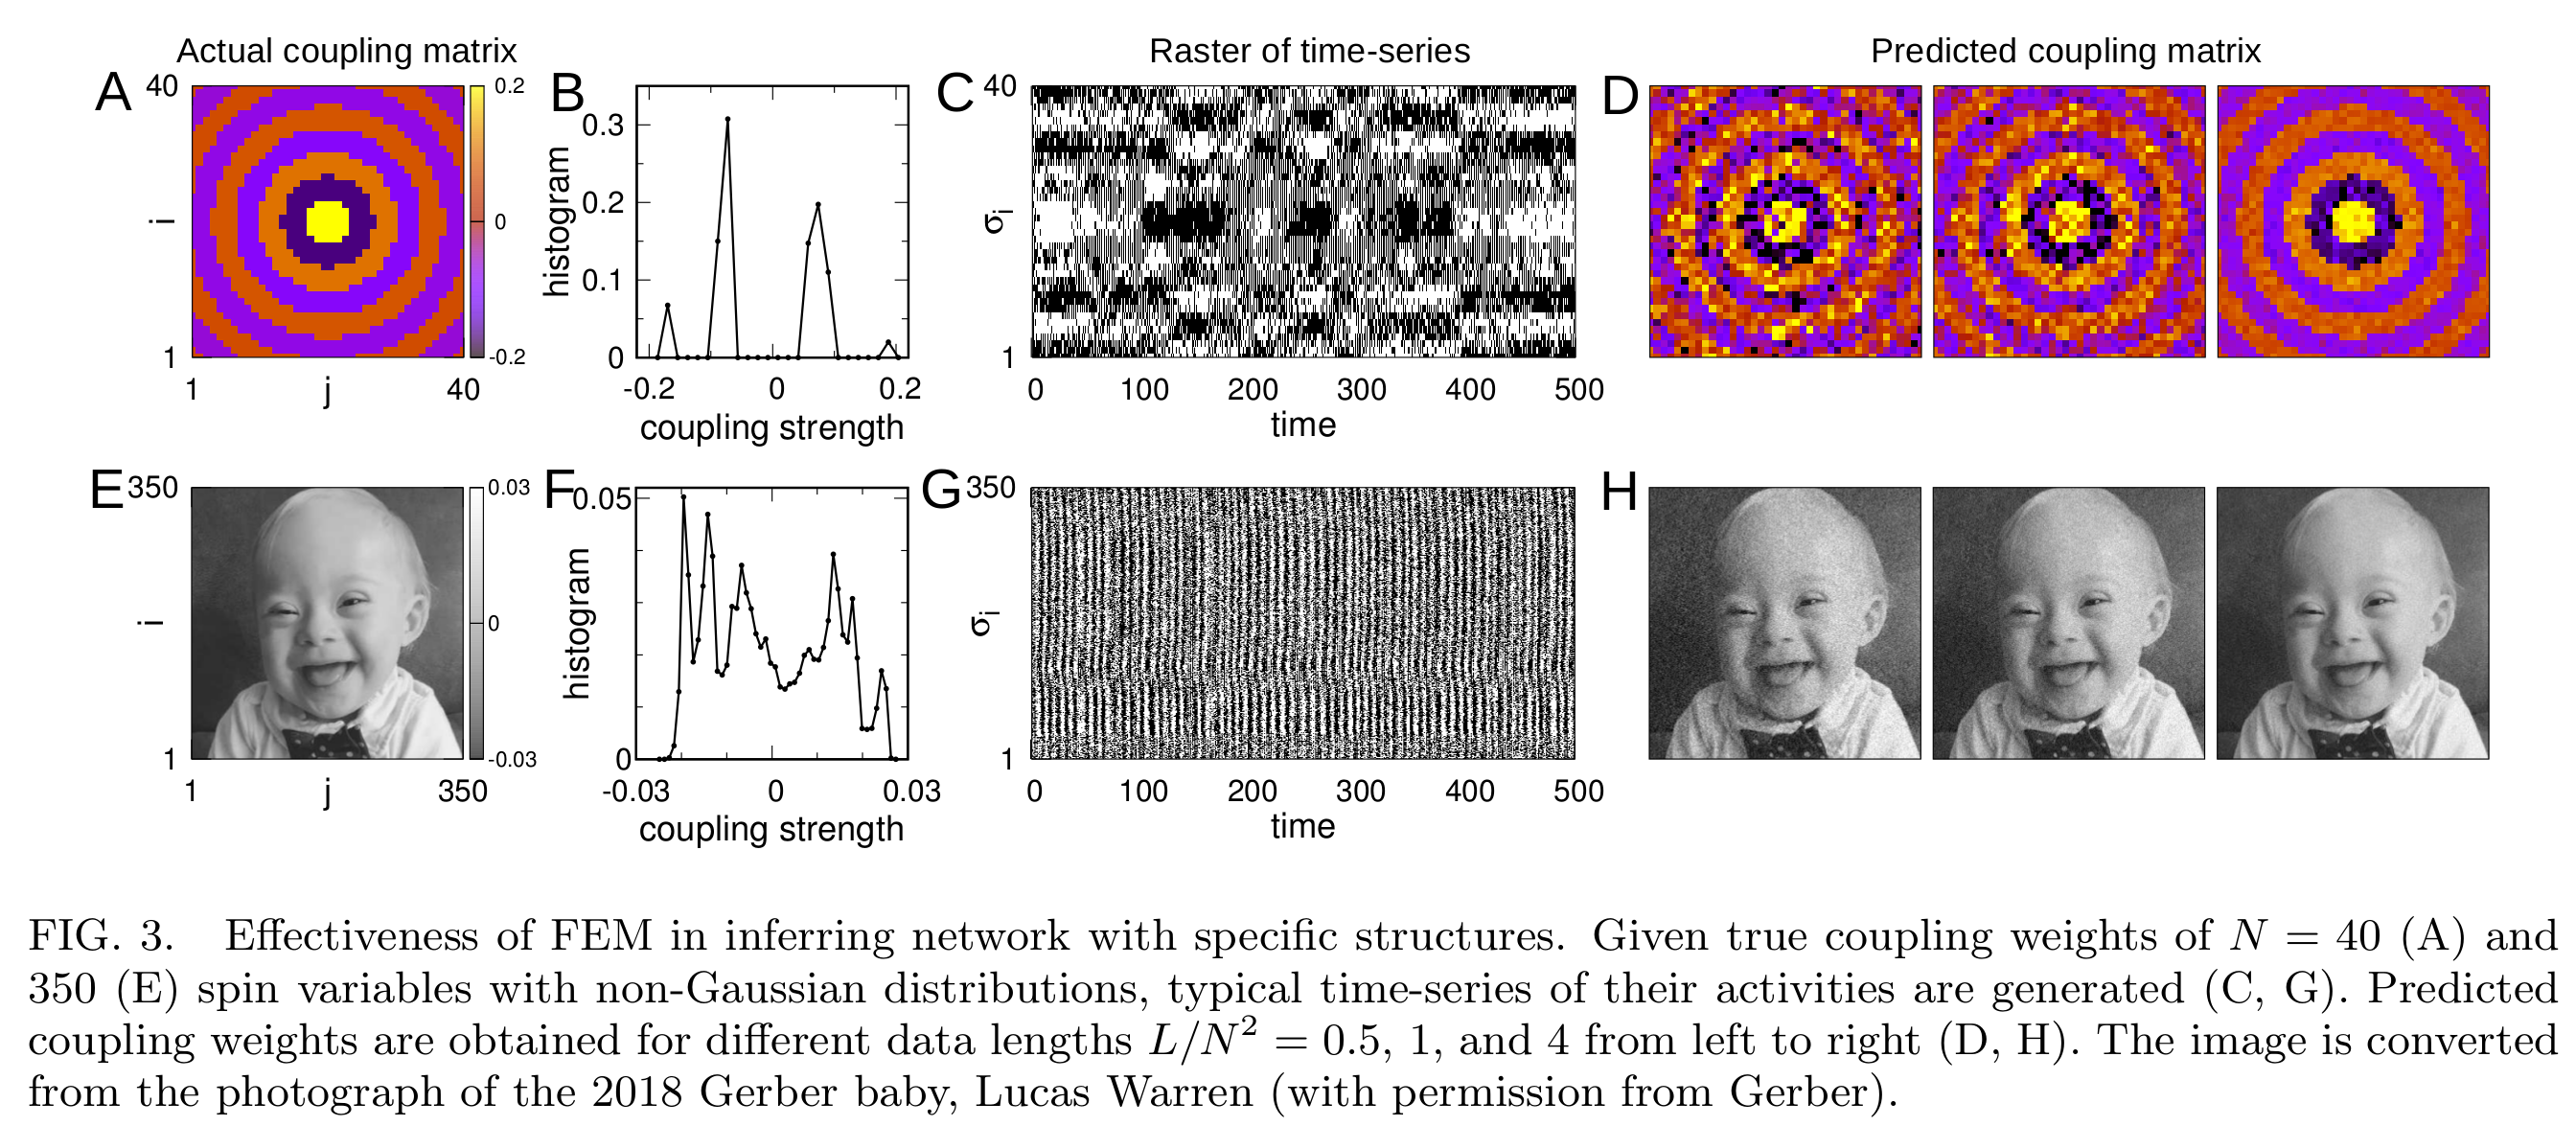
\includegraphics[width=16cm]{fig1}
\caption{ \label{fig:fig1}Network inference for the kinetic Ising model. Inference error (MSE, black) and discrepancy ($D$, gray) are shown as function of number of iterations for large observed configurations, $L/N^2=1$ (A) and few observed configurations, $L/N^2=0.2$ (C). Predicted couplings versus actual couplings for $L/N^2=1$ (B) and $L/N^2=0.2$ (D). The inference errors are obtained for na\"ive mean-field (nMF), Thouless-Anderson-Palmer (TAP), exact mean-field (eMF), Maximum Likelihood Estimation (MLE), and Free Energy Minimization (FEM), for various number of observed configurations, $L/N^2$ from $0.2$ to $1$ in the limit of weak coupling, $g=1$ (E), and in the limit of stronger coupling, $g=2$ (F), $g=3$ (G), and $g=4$ (H). A system size $N=100$ is used. A learning rate $\alpha=1$ is used for MLE.
}
\end{figure*}

\section{Results}
\subsection{Kinetic Ising model}
We first tested FEM on the inference of connection weights $W_{ij}$ ($\neq W_{ji}$) in the kinetic Ising model, which is often used as a benchmark for stochastic causality inference.
The Sherrington-Kirkpatrick (SK) model assumes $W_{ij}$ are normally distributed with zero mean and variance equal to $g^2/N$~\cite{Sherrington1975}.
%Our iterative method could successfully infer true $W_{ij}$ (Fig.~\ref{fig:fig1}A).
% Inference in under-determined problems must include some criterion to avoid over-fitting.
In the limit of large sample size (large $L/N^2$), our iterative method decreases the mean square error, 
MSE = $N^{-2} \sum_{i,j=1}^N (W_{ij} - W_{ij}^{\textrm{true}})^2$, as the number of iterations increases (Fig.~\ref{fig:fig1}A).
We obtain good agreement between true and predicted weights (Fig.~\ref{fig:fig1}B).
In real world problems, $W_{ij}^{\textrm{true}}$ is inaccessible so MSE cannot be defined.
However, $D_i(W)$ in Eq.~(\ref{eq:D}) is an alternative measure of the discrepancy between observation $\sigma_i(t+1)$ and model expectation.
The discrepancy measures $D_i(W)$ are independent for each spin $i.$ 
%In real problems, however, the true $W_{ij}^{\textrm{true}}$ is unknown, therefore MSE is unobtainable. 
%One can stop the iteration after a "large enough" number of iterations. This is not clear what is large enough because this number depends on data. A too large number of iterations cannot improve the prediction result but needs an expensive computation.  Instead, the discrepancy $D_i(W)$ in Eq.~(\ref{eq:D}) can be a data-driven probe that measures the discrepancy between observation $\sigma_i(t+1)$ and its expectation. (Fig.~\ref{fig:fig1}A). Therefore, stopping the iteration when $D_i(W)$ saturates can induce a good prediction with an optimal computational time.
We checked that MSE and $D=N^{-1}\sum_{i=1}^N D_i(W)$ change similarly during iterations.
More importantly, for small sample sizes (small $L/N^2$), MSE and $D$ decrease  with iterations initially, 
but start to increase after some number of iterations (Fig.~\ref{fig:fig1}C). 
For the kinetic Ising model, $D_i(W)=4\sum_{t} [1-P(\sigma_i(t+1)|\sigma(t))]^2$ 
with the transition probability, $P(\sigma_i(t+1)|\sigma(t))$ in Eq.~(\ref{eq:kIsingProb}).
Therefore, decreasing $D_i(W)$ can only result from $P(\sigma_i(t+1)|\sigma(t))$ saturating the causal relation between observations, $\sigma(t)$ and $\sigma_i(t+1)$, through $W.$ Distinct spins indexed by  $i$ often require different numbers of iterations.
%Therefore, $D(W)$  provides an effective stopping criterion not only to avoid unnecessary computation for large $L/N^2$,
%but also to avoid over-fitting for small $L/N^2$.
%Therefore, stopping the iteration at the minimal $D_i(W)$ can avoid over-fitting for small $L/N^2$.
Stopping the iteration for spin $i$ when $D_i(W)$ saturates leads to accurate inference with minimal computation.
For limited data (e.g. $L/N^2 = 0.2$), these stopping criteria lead to accurate inference (Fig.~\ref{fig:fig1}D) without over-fitting.
%Since $\sigma_i(t+1)$ has spin index $i$ in the kinetic Ising model, we consider 
%Our iterative method could successfully infer true couplings $W_{ij}$ not only in the limit of large observed configurations (Fig.~\ref{fig:fig1}B) but also in the limit of few observed configurations (Fig.~\ref{fig:fig1}D). 
%{\color{red} Should we exchange the position of figure B and C?}

Now we compare the inference performance of our method with other representative methods~\cite{Roudi2011, Mezard2011, Zeng2013}: na\"ive mean field (nMF), Thouless-Anderson-Palmer mean field (TAP), exact mean field (eMF), and maximum likelihood estimation (MLE). 
%{\color{blue}((I think MLE is more correct than MAP because we don't consider prior to compute posterior))}
MLE requires maximizing the data likelihood, ${\cal P} = \prod_{t=1}^{L-1} \prod_{i=1}^N P(\sigma_i(t+1)|\sigma(t))$, and uses gradient ascent to update $W_{ij}$ incrementally through $W^{\textrm{new}}_{ij} = W_{ij} + {\alpha}/({L-1}) {\partial \log {\cal P}}/{\partial W_{ij}}$~\cite{Roudi2011, Zeng2013},
%\begin{equation}
%W^{new}_{ij} = W_{ij} + \frac{\alpha}{L-1} \frac{\partial \log {\cal P}}{\partial W_{ij}},
%\end{equation}
where the learning rate $\alpha$ is an undetermined parameter controlling the updating speed.
In contrast, the maximizing condition ($\partial \log {\cal P}/{\partial W_{ij}}=0$) and mean-field approximations provide matrix equations,
$W=A^{-1}BC^{-1}$, where matrices $B_{ij} = \langle \delta \sigma_i(t+1) \delta \sigma_j(t) \rangle$ and $C_{ij}= \langle \delta \sigma_i(t) \delta \sigma_j(t) \rangle$ represent time-delayed and equal-time correlations in data, and $A$ are diagonal matrices, which are different for nMF, TAP, and eMF (SI Text 2 has brief reviews of these mean-field methods).
%although various mean-field methods work perfectly for weak coupling and sufficient data regimes (refs).
%The MAP maximizes the likelihood, ${\cal P} = \prod_{t=1}^{L-1} \prod_{i=1}^N P(\sigma_i(t+1)|\sigma(t))$, with respect to $W_{ij}$.
%Using the gradient descent method, one can iteratively update $W_{ij}$:
%By construction, the MAP estimate converges to the true probabilities in the large $L$ limit.

For weak coupling ($g=1$), TAP, eMF, MLE and FEM have similar inference accuracy that increases with sample size (Fig.~\ref{fig:fig1}E).
nMF showed poor accuracy independent of data size, since the zeroth-order mean-field approximation works only for very weak coupling strengths~\cite{Roudi2011}.
As we further increase coupling strength, the other two mean-field methods, TAP and eMF also start to give less accurate results than MLE and FEM (Fig.~\ref{fig:fig1}F-H). 
For large sample size ($L/N^2>1$), our iterative method, FEM, works as well as standard MLE. For small sample size, however, FEM provides better accuracy than MLE.
For example, the inference error (MSE) of FEM is approximately 4 times lower than that of MLE for $L/N^2=0.2$ and $g=4.$
% while nMF does not converge. The nMF works only in the limit of very large number of observed configurations and very weak coupling (Ref).  When the coupling increases, TAP and eMF could not converge, MAP also started to diverse in the limit of very few observed configurations (Fig.~\ref{fig:fig1}F-H). For instance, with $L/N=0.2$ and $g=4$, MSE obtained using our method is approximately 4 times lower than that using MAP inference.
%Unlike a parameter-free approach as our method, the MAP estimation does not converge with a large learning rate, i.e., $\alpha = 3$. The result from MAP is getting better with $\alpha = 1$. The lower $\alpha = 0.5$ induces the same result with $\alpha = 1$  (Fig.Sxx). 
%More detail, in the limit of weak coupling variability ($g=2$) and a large number of observed configurations ($L/N^2=1$), FEM works as well as MAP. However, in the limit of strong coupling variability ($g=4$) and/or smaller numbers of observed configurations ($L/N^2=0.2$), our method provided much better accuracy (Fig.~\ref{fig:fig1}F). For $L/N=0.2$ and $g=4$, MSE obtained using our method is approximately 4 times lower than that using MAP inference.
In addition to inference accuracy, FEM has two advantages in computation. %, although both FEM and MLE are iteration-based methods.
First, the FEM update is multiplicative and not incremental, while MLE updates (using conjugate gradient ascent or some other numerical maximization) have an undetermined parameter, the learning rate $\alpha,$ which needs to be determined.
A very large rate ($\alpha=3$) leads to loss of convergence, whereas a very small rate ($\alpha=0.5$) leads to many iterations with infinitesimal updates. We set $\alpha=1$.
Second, FEM requires 20 times fewer updates than MLE (Fig.~\ref{fig:figS1}A), which reduces computation time a 100-fold (Fig.~\ref{fig:figS1}B).
%leads to 100 times less computation time in our hands (Fig.~\ref{fig:figS1}B).
%{\color{blue}((If we have a page-limit problem, we may move Fig. 2 as a Supplementary Figure))}

\begin{figure}[h]
\centering
\includegraphics[width=9cm]{figS1}
\caption{ \label{fig:figS1} Efficiency of inference. Number of iterations per spin (A) and real computational time (B) by using MLE versus FEM for various coupling strengths, $g$ from $1$ to $4$ and number of observed configurations, $L/N^2$ from $0.2$ to $1$. A system size $N=100$ is used. A learning rate $\alpha=1$ is used for MLE.
}
\end{figure}

%It is worth noting that unlike parameter-free approach as our method, the MAP estimation has a turning parameter, learning rate $\alpha$. Selecting an optimal value of $\alpha$ is not trivial, a large value (i.e., $\alpha = 3$) caused a divergence of this method. A very small value of learning rate (i.e., $\alpha = 0.5$) induced a very expensive in computational time. Here We selected $\alpha = 1$ to show the performance of MAP.
%For more detail, we compared the number of iterations per spin and computation time for MAP with $\alpha = 1$ and FEM. FEM required about 20 times less iterations than MAP (Fig.~\ref{fig:fig2}A). Furthermore, FEM was about 100 times faster in real computation time (Fig.~\ref{fig:fig2}B).
\begin{figure*}
\centering
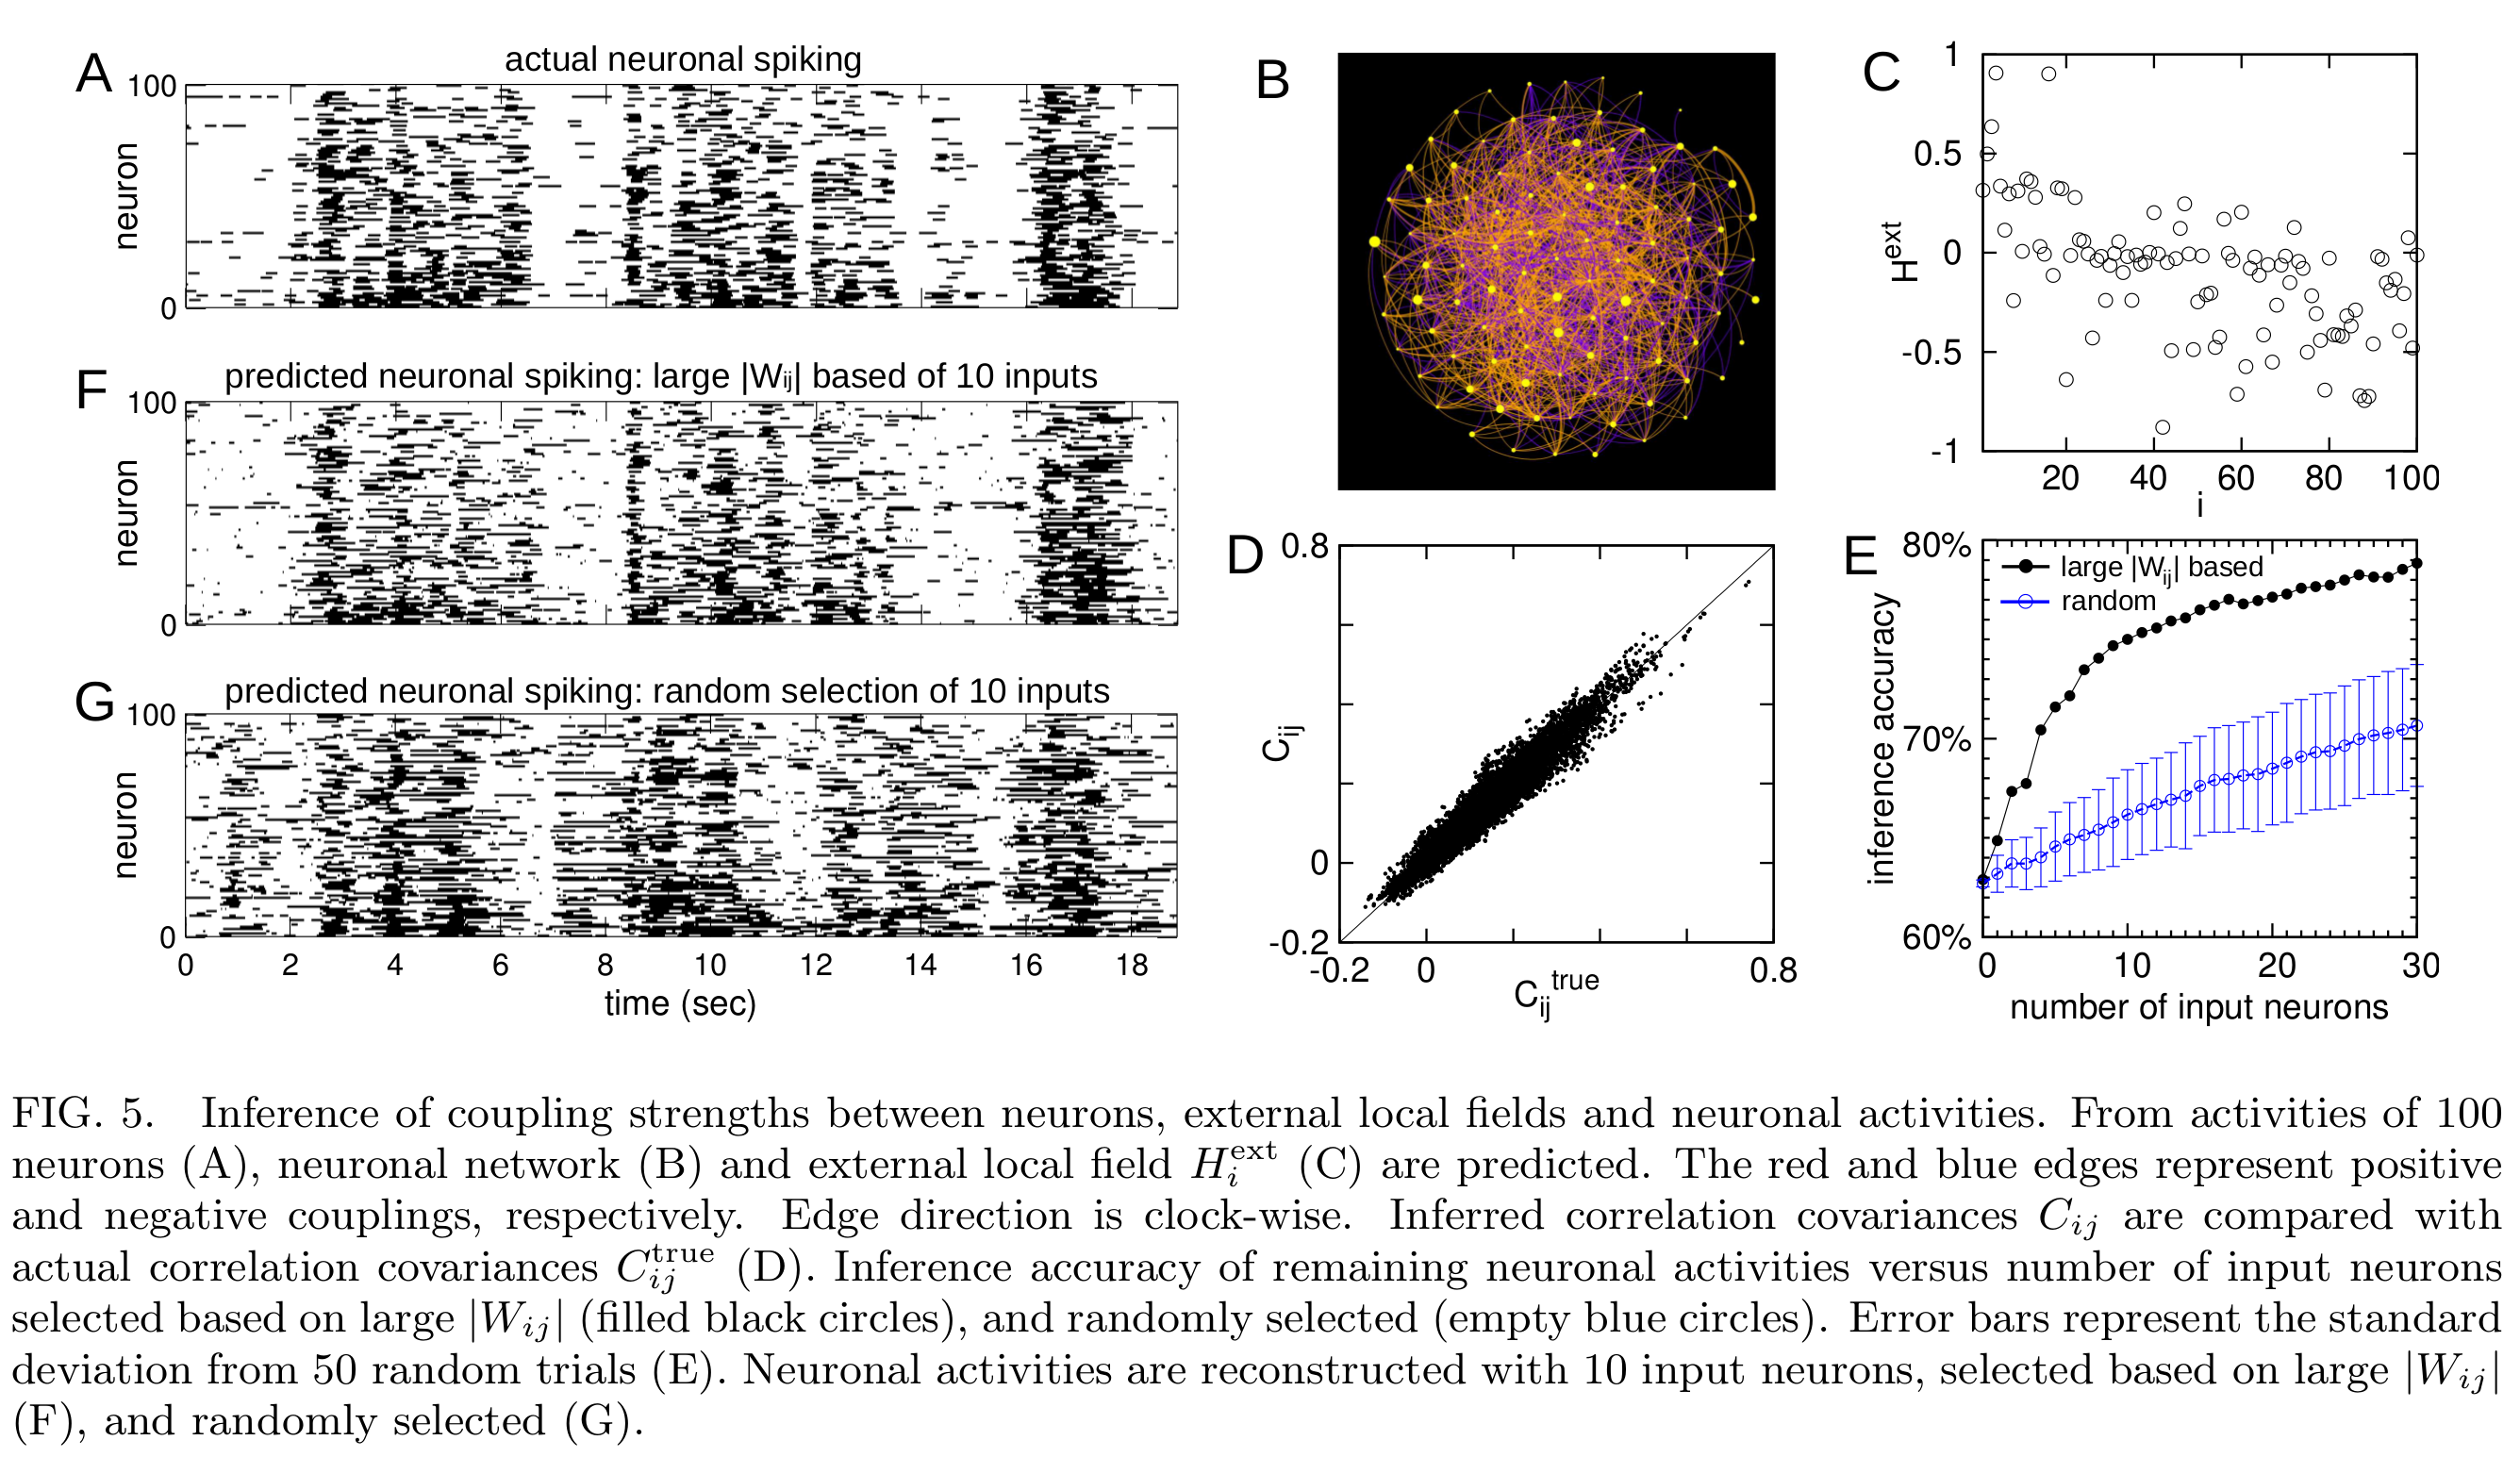
\includegraphics[width=16cm]{fig2}
\caption{ \label{fig:fig2}Effectiveness of FEM in inferring network with specific structures. Given true coupling weights of $N=40$ (A) and  $350$ (E) spin variables with non-Gaussian distributions, typical time-series of their activities are generated (C, G). Predicted coupling weights are obtained for different data lengths $L/N^2=0.5$, $1$, and $4$ from left to right (D, H). The image is converted from the 2018 Gerber baby's photograph (with permission from Gerber).
}
\end{figure*}

\begin{figure}
\centering
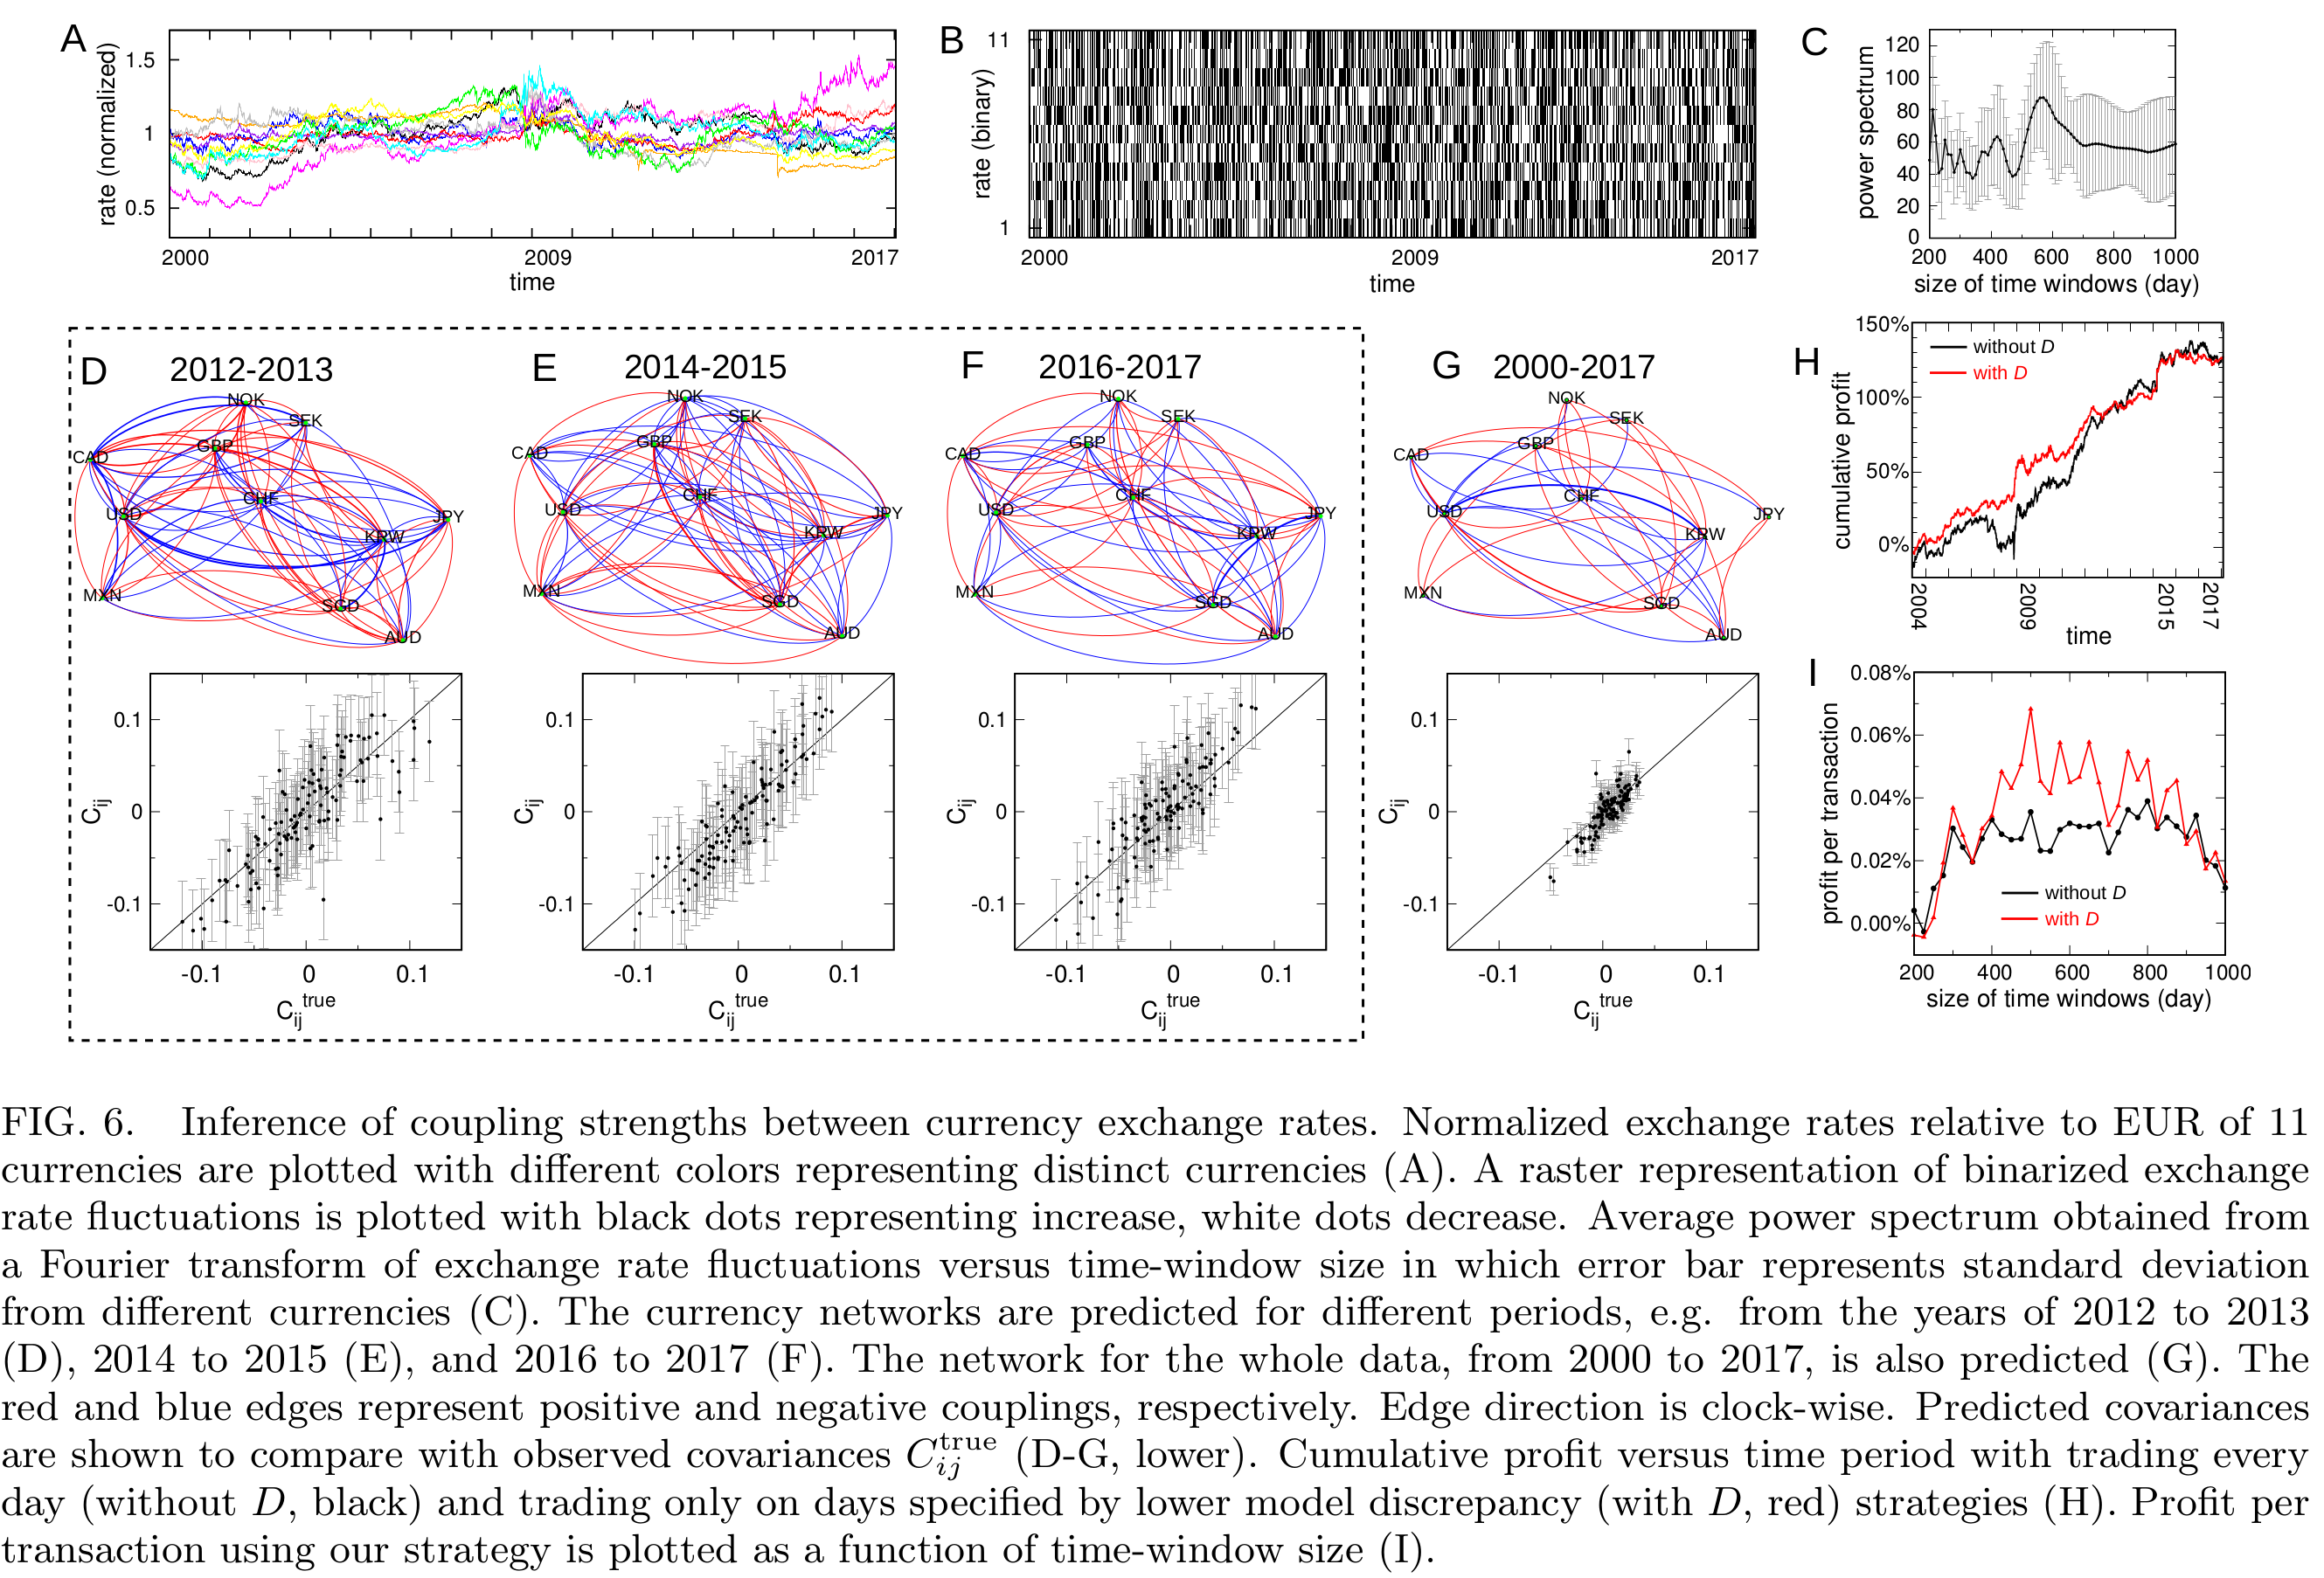
\includegraphics[width=8.cm]{fig3}
\caption{ \label{fig:fig3}Accurate inference of higher-order coupling strengths.
Linear (A) and quadratic (B) coupling strengths in the nonlinear kinetic Ising model %with the local field, 
%$H_i(\sigma(t))=\sum_j W_{ij} \sigma_j(t) + \sum_{j,k} Q_{ijk} \sigma_j(t) \sigma_k(t)/2$, 
are predicted from FEM. Here the true coupling strengths are normally distributed with a system size $N=40$.
Three different data lengths, $L=1.6\times10^4$ (gray), $6.4\times10^4$ (blue) and $2.56\times10^5$ (red), are examined. 
}
\end{figure}


To further demonstrate the effectiveness of FEM, we show two examples of inferred networks when $W_{ij}$ has more general coupling distributions than the SK model, as real systems often deviate strongly from normally-distributed coupling strengths.
In the first example, the spins have alternating bands of positive and negative couplings modulated by distance as $|W_{ij}| = W_{0}/\log(R_{ij})$, where $R_{ij}$ represents the radius of the circle (Fig.~\ref{fig:fig2}A). The couplings are non-normally distributed (Fig.~\ref{fig:fig2}B). The spin raster scan exhibits nontrivial structure (Fig.~\ref{fig:fig2}C), reminiscent of binocular rivalry~\cite{Moreno-Bote:2007a}. 
As the number of observed configurations increases, the predicted coupling strengths (Fig.~\ref{fig:fig2}D) approach their true values (Fig.~\ref{fig:fig2}A).
%In the second, the spins are in blocks of positive and negative couplings (Fig.~\ref{fig:fig2}D) with no obvious structure in the simulated spin raster scan (Fig.~\ref{fig:fig2}E), but the coupling strength (Fig.~\ref{fig:fig2}F) are still predicted well.
In the second, the 2018 Gerber baby's photograph was used as the heatmap of the coupling matrix (Fig.~\ref{fig:fig2}E). These couplings are also non-normally distributed (Fig.~\ref{fig:fig2}F) with periodic bursting in the simulated spin raster scan (Fig.~\ref{fig:fig2}G), but the couplings are still predicted well (Fig.~\ref{fig:fig2}H).


Our formulation, based on the differential geometry of the data free energy, automatically includes higher-order regression equations for the local field $H_i (\sigma)$ (SI Text 1).
%For example, when the local field has both linear and quadratic terms, $H=W\sigma + Q \sigma^2/2$, the corresponding regression equations are $Q = \langle \delta H \delta \sigma \delta \sigma \rangle \langle \delta \sigma \delta \sigma \rangle^{-2} - \langle \delta H \delta \sigma \rangle \langle \delta \sigma \delta \sigma \delta \sigma \rangle \langle \delta \sigma \delta \sigma \rangle^{-3}$ and $W = \langle \delta H \delta \sigma \rangle \langle \delta \sigma \delta \sigma \rangle^{-1} - Q \langle \sigma \rangle.$ 
For example, we checked higher-order inference with FEM by using a generalized kinetic Ising model with linear and quadratic couplings, $H_i(\sigma(t))=\sum_{j} W_{ij}\sigma_{j}(t) + \sum_{j,k} Q_{ijk} \sigma_j(t)\sigma_k(t)/2$, where $W_{ij}$ and $Q_{ijk}$ are normally distributed. The quadratic couplings are symmetric ($Q_{ijk} = Q_{ikj}$) and have no self-interactions ($Q_{ijj}=0$) since $\sigma_j^2 = 1.$ The number of $Q_{ijk}$ parameters is $N^2(N-1)/2.$ 
The recovery of both linear and quadratic couplings is evident (Fig.~\ref{fig:fig3}).


\begin{figure*}
\centering
\includegraphics[width=15cm]{fig4}
\caption{\label{fig:fig4} Inference of coupling strengths between neurons, external local fields and neuronal activities. From activities of 100 neurons (A), neuronal network (B) and external local field $H_i^{\textrm{ext}}$ (C) are predicted. The red and blue edges represent positive and negative couplings, respectively. Edge direction is clock-wise. Inferred correlation covariances $C_{ij}$ are compared with actual correlation covariances $C_{ij}^{\text{true}}$ (D). Inference accuracy of remaining neuronal activities versus number of input neurons selected based on large $|W_{ij}|$ (filled black circles), and randomly selected (empty blue circles). Error bars represent the standard deviation from 50 random trials (E). Neuronal activities are reconstructed with 10 input neurons, selected based on large $|W_{ij}|$ (F), and randomly selected (G).}
%, in comparison with actual data (E). Black dots represent spikes, white dots present silences.}
%Inference of coupling strengths between neurons, external local fields and neuronal activities. Raster of $100$ neuronal activities from pre-processing (A) and processing (B) data are plotted in which black dots represent spikes, white dots present silences. Coupling from neuron $j$ to neuron $i$ (C) and external local field $H_i^{\textrm{ext}}$ (D) are predicted from our method. Inferred correlation covariances $C_{ij}$ are shown to compare with actual correlation covariances $C_{ij}^{\text{true}}$ (E). Inference accuracy of remaining neuron activities versus number of input neurons (F) under our selection, large $|W_{ij}|$ based (filled black circles), and under random selection (empty blue circles). Error bars represent the standard deviation from 50 random trials. neuronal activities are reconstructed with 10 input neurons under our selection, large $|W_{ij}|$ based (G), and under random selection (H).}
\end{figure*}

\subsection{Neuronal network}
We applied our method to infer a neuronal network from temporal neuronal activities in the tiger salamander ({\it Ambystoma tigrinum}) retina~\cite{Marre2017}.
The multi-channel experiment recorded stochastic firing patterns of 160 neurons when the salamander retina was stimulated by a film clip of fish swimming. 
%The natural movie duration is $19$ s and the experiment was repeated $297$ times. 
As in Ref.~\cite{Tkacik2014}, %\cite{Marre2017}, 
we considered only the 100 most active neurons. % (Fig.~\ref{fig:fig5}E).
%In the original data, neuron $i$ is defined as ``active'' ($\sigma_i(t) = 1$), if the neuron fires at least once during the time window $[t, t+\delta t]$, otherwise ``silent'' ($\sigma_i(t)=-1)$ (Fig.~\ref{fig:fig5}A).
%To suppress the dependency of the time interval $\delta t$ for the activity definition, we used a moving average of activities.
%[Explain the data processing in the Supplemental text!!]
%We examined the past five and future five activities of neuron $i$, and redefined $\sigma_i(t)=1$, if neuron $i$ emitted at least one spike in the time window, otherwise $\sigma_i(t)=-1$ (Fig.~\ref{fig:fig5}B).
%Since neurons may have a refractory period that prevents consecutive spikes after emitting a spike~\cite{Kara2000}, the moving average can also help infer the genuine interaction between neurons by reducing the effect of the refractory period.
%Using the processed time-sequence data, 
After processing the data (SI Text 3; Fig.~\ref{fig:fig4}A), we inferred the neuronal network governing the local field, $H_i(\sigma(t))=H_{i}^{\textrm{ext}} + \sum_{j} W_{ij}\sigma_{j}(t)$.
Here we included a constant bias external field $H_{i}^{\textrm{ext}}$ for neuron $i$ to consider the persistent silence of neurons.
%We estimated the connection weights $W_{ij}$ %from neuron $j$ to neuron $i$ 
We inferred the neuronal network weights $W_{ij}$ (Fig.~\ref{fig:fig4}B), and the external local fields for each neuron by using $H_{i}^{\textrm{ext}} = \langle H_i \rangle - \sum_{j} W_{ij} \langle \sigma_{j} \rangle $.  
%{\color{blue}((Please check this sentence for explaining how you estimated the external fields))}
The external local fields are mostly negative, which implies that neuronal activities are biased to be silent (Fig.~\ref{fig:fig4}C).

The true couplings are unknown for this system. As a  validation, with the $H_{i}^{{\textrm{ext}}}$ and $W_{ij}$ we determined, we simulated neuronal activities. %by using the local field $H_i(\sigma(t)).$
We found agreement between the covariances of neuronal activities $C_{ij}= \langle \delta \sigma_i(t) \delta \sigma_j(t) \rangle$ 
of the observed and simulated data (Fig.~\ref{fig:fig4}D).
For a more stringent validation, we reconstructed the full neuronal activities from specific `pinned' neuron activities, representing inputs.
Fixing the time sequences $\sigma_j(t)$ of specific chosen input neurons $j \in I$, we reconstructed the activities $\sigma_i(t+1)$ of the remaining neurons $i \not\in I$. %, using the local field {\color{red} $H_i(\sigma(t))=H_i^{\text{ext}} + \sum_{j} W_{ij} \sigma_j(t)$}.
 %$H_i(\sigma(t))=H_i^{\text{ext}} + \sum_{j \in I} W_{ij} \sigma_j(t)$.
As a control, we selected the input neurons at random and compared them with input neurons selected on the basis of the coupling strength $|W_{ij}|$ as the input set $I.$
As more input neurons are considered, the reconstruction predicts $\sigma_i(t+1)$ more accurately (Figs.~\ref{fig:fig4}E and~\ref{fig:figS3}). %(Fig.~\ref{fig:fig4}E; Fig. S2).
%The reconstruction is considerably more accurate  when the  neurons are pinned.
 Pinning the activities of only $|I|=10$ strongly coupled neurons gave predicted activities of the remaining 90 neurons that were very close to the observed activities (Fig.~\ref{fig:fig4}F), in contrast to predicted activities obtained by pinning randomly selected sets of 10 input neurons (Fig.~\ref{fig:fig4}G).

\subsection{Currency network}

Finally, we apply our method to another difficult and representative stochastic problem, currency exchange rate fluctuations.
We obtained time series of currency exchange rates from January 2000 to December 2017~\cite{BankItaly}, and examined exchange rates denominated in Euro (EUR) %{\color{red} (the amount of foreign currencies for 1 EUR)} 
of $11$ actively traded currencies (Fig.~\ref{fig:fig5}A). %: US dollar (USA), Canadian dollar (CAD), Mexican perso (MXN), British pound sterling (GBP), Norwegian krone (NOK), Swiss franc (CHF), Swedish krona (SEK),  Australian dollar (AUD), Japanese yen (JPY), South Korean won (KRW),  and Singapore dollar (SGD), excluding currencies that are highly correlated with these currencies, e.g., Hong Kong dollar (HKD) versus USD, and New Zealand dollar (NZD) versus AUD (Fig.~\ref{fig:fig6}A). %.The exchange rates of these currencies fluctuated during the time Using this currency data, we examine whether our inference method can work for coarse-grained data and for time-dependent couplings between stochastic variables. 
First, we concentrate on the daily fluctuations of the exchange rates, since most financial analyses center on price increments rather than absolute prices~\cite{Pincus2004}.
We binarize the real-valued rates to concentrate on the sign of their daily fluctuations (Fig.~\ref{fig:fig5}B).
We defined the binarized rate $\sigma_i(t)=1$ for a day-to-day increase of exchange rate $i$ at time $t$ ($r_i(t) > r_i(t-1))$,
and $\sigma_i(t)=-1$ for the decrease. If there was no change ($r_i(t) = r_i(t-1)$), we set $\sigma_i(t)=\sigma_i(t-1)$.
Second, we divide the data for different periods to investigate the time dependence of the couplings between exchange rates.
Using the Fourier transform of the binarized time series, we identified a characteristic period, 550 business days ($\sim$ 2 years), of the fluctuations (Fig.~\ref{fig:fig5}C). 
We inferred the currency network weights $W_{ij}$ separately in two year periods, shown here (Figs.~\ref{fig:fig5}D-F, upper) for the three periods  2012-2013, 2014-2015, and 2016-2017.
%($H_i^{\text{ext}}$ was negligible.)
We found agreement between the covariance $C_{ij}=\langle \delta \sigma_i(t) \delta \sigma_j(t) \rangle$ of the observed currency data and that of the simulated currency data using $H_i(\sigma(t))=H_{i}^{\textrm{ext}} + \sum_{j} W_{ij}\sigma_{j}(t)$ (Figs.~\ref{fig:fig5}D-F, lower).
In contrast, when we estimated the currency network using the data for the entire period 2000-2017, the network had weaker connections and smaller covariances $C_{ij}$ compared to the time-dependent analysis (Figs.~\ref{fig:fig5}G)

The raw exchange rate data is continuous. Is our binarized inference of any practical value? To address this, we simulated a currency trade strategy, and checked if the strategy was profitable. Using only data within a time window of a period $T$,  $\{\sigma(t-T+1), \sigma(t-T+2), \cdots, \sigma(t) \},$
we predicted the currency fluctuations $\sigma(t+1)$ on the next day.
For the trade simulation, we considered a hedging trader who buys one currency with 1 EUR and sells one currency with 1 EUR.
To earn profits, the trader is supposed to sell/buy a currency that has the highest probability of increase/decrease in exchange rate:
the currency $sell = \arg\max_i P(\sigma_i(t+1)=+1|\sigma(t))$  and the currency $buy = \arg\max_i P(\sigma_i(t+1)=-1|\sigma(t))$.
Then, a daily profit can be defined as ${\text{profit} (t)} = r_{sell}(t+1)/r_{sell}(t) - r_{buy}(t+1)/r_{buy}(t)$.
We calculated cumulative profits of the trade simulation from 2004 to 2017 with various time window sizes that we considered as past information (Fig.~\ref{fig:fig5}H for $T = 500$ days). 
%{\color{blue}((Logically it would be better to switch Fig. 6H and Fig. 6I))}
Hedging strategies profit from market volatility and, indeed, our trade simulation showed large profits when the exchange rates had large fluctuations (Fig.~\ref{fig:fig5}A).
The window size $T$ had an optimal period of 500-750 business days (Fig.~\ref{fig:fig5}I).
For a more refined strategy, we considered the quality or accuracy of our inference by probing the discrepancy $D_i(W)$ in Eq.~(\ref{eq:D}).
Instead of trading every day, we traded only on the days when the discrepancy at that day, %$D(t) \equiv \sum_{i} \big[ \sigma_i(t) - \tanh H_i(t-1) \big]^2$, 
$D(t) \equiv \sum_{i} \big[ \sigma_i(t) - \langle \langle \sigma_{i}(t) \rangle \rangle _{\sigma(t-1)} \big]^2$, was lower than the average $T^{-1} \sum_{t=1}^T D(t)$ for a fixed window size $T$. %This  reduced the number of transactions by approximately half and
% $D(W)$ was lower than the average $D(W)$ for a fixed window size $T$.
This strategy doubled the profits per transaction (Figs.~\ref{fig:fig5}H and \ref{fig:fig5}I), showing that the discrepancy $D_i(W)$ is a useful measure of model accuracy. 

    
\begin{figure*}
\centering
\includegraphics[width=15cm]{fig5}
\caption{ \label{fig:fig5}Inference of coupling strengths between currency exchange rates. Normalized exchange rates relative to EUR of 11 currencies are plotted with different colors representing distinct currencies (A). A raster representation of binarized exchange rate fluctuations is plotted with black dots representing increase, white dots  decrease. Average power spectrum obtained from a Fourier transform of exchange rate fluctuations versus time-window size in which error bar represents standard deviation from different currencies (C). The currency networks are predicted for different periods, e.g. from the years of 2012 to 2013 (D), 2014 to 2015 (E), and 2016 to 2017 (F). The network for the whole data, from 2000 to 2017, is also predicted (G). The red and blue edges represent positive and negative couplings, respectively. Edge direction is clock-wise. Predicted covariances are shown to compare with observed covariances $C_{ij}^{\text{true}}$ (D-G, lower). Cumulative profit versus time period for various time-window sizes (H). Profit per transaction using our strategy is plotted as a function of time-window size (I).  
}
\end{figure*}    
    
    
\section{Discussion}
We demonstrated that under-determined stochastic systems can be inferred in a conceptually simple and computationally efficient manner using the mathematical framework of statistical physics.
Since network inference is an important subject, many different approaches have been developed.
Equilibrium approaches assume symmetric interactions ($W_{ij}=W_{ji}$) between node $i$ and node $j$, and estimate the pair-wise interaction strengths that can maximally explain the observed static patterns of network activity in brains~\cite{Tkacik2014, Tkacik2015, Watanabe2013}, proteins~\cite{Mora2010, Weigt2009}, and stock markets~\cite{Bury2012}.
In contrast, non-equilibrium approaches do not assume symmetry, and infer asymmetric causal relations between nodes that can better explain  dynamic patterns of network activity~\cite{Zeng2013}.
Causality inference for non-equilibrium models (e.g., using recurrent neuronal networks) is computationally expensive.
Although mean-field methods have been introduced to circumvent this practical problem~\cite{Roudi2011}, these approximation methods only work for weak-interaction regimes with large sample size.
All small sample size inference must contend with over-fitting so the key feature of our approach was to consistently decouple the model update step and a discrepancy measure that is similar to Expectation Maximization. This decoupling allowed us to iterate with a multiplicative model update, and to stop when the discrepancy measure quantifies that the multiplicative update has saturated. 
We derived this within a standard statistical physics formulation~\cite{schwinger1953,toms2007schwinger},
so no ad hoc averaging or approximation steps were involved. We demonstrated that our method outperfoms others in inferring the asymmetric interactions of the kinetic Ising model, especially in strong-interaction regimes, and particularly when available data was limited. 
Another aspect of small sample size inference is that longer time-scale modulation of couplings can be uncovered. This is of considerable practical import as we demonstrated with the currency exchange rate network.

FEM has several computational merits. Besides having no incremental learning rate that requires tuning, %it is embarrassingly 
the method is parallelizable and scalable:
We computed results for the kinetic Ising model with up to $N=5000$ interacting spins, determining $2.5 \times 10^7$ parameters (Fig.~\ref{fig:figS4}).
We also demonstrated that the method can infer not only linear interactions but also higher-order interactions.
Moreover, FEM is generalizable to systems with any number of discrete states, although we focused on binary stochastic systems here.
Uncovering hidden nodes for stochastic network inference~\cite{Hoang2018} is an exciting avenue for future work.

%\begin{table}%[tbhp]
%\centering
%\caption{Comparison of the fitted potential energy surfaces and ab initio benchmark electronic energy calculations}
%\begin{tabular}{lrrr}
%Species & CBS & CV & G3 \\
%\midrule
%1. Acetaldehyde & 0.0 & 0.0 & 0.0 \\
%2. Vinyl alcohol & 9.1 & 9.6 & 13.5 \\
%3. Hydroxyethylidene & 50.8 & 51.2 & 54.0\\
%\bottomrule
%\end{tabular}
%\addtabletext{nomenclature for the TSs refers to the numbered species in the table.}
%\end{table}

\section*{Acknowledgment}
Ga\v{s}per Tka\v{c}ik  generously provided the neuronal activity data. We thank Changbong Hyeon and Arthur Sherman for comments on the manuscript.
This work was supported by Intramural Research Program of the National Institutes of Health, NIDDK (D.-T.H.,V.P.), and by Basic Science Research Program through the National Research Foundation of Korea (NRF) funded by the Ministry of Education (2016R1D1A1B03932264) and the Max Planck Society, Gyeongsangbuk-Do and Pohang City (J.J.).

\bibliography{pnas-network}

clearpage
%\pagebreak
%\newpage
%%%%%%%%%% Merge with supplemental materials %%%%%%%%%%
%%%%%%%%%% Prefix a "S" to all equations, figures, tables and reset the counter %%%%%%%%%%
\setcounter{equation}{0}
\setcounter{figure}{0}
\setcounter{table}{0}
\setcounter{page}{1}
\makeatletter
\renewcommand{\theequation}{S\arabic{equation}}
\renewcommand{\thefigure}{S\arabic{figure}}
%\renewcommand{\bibnumfmt}[1]{[S#1]}
%\renewcommand{\citenumfont}[1]{S#1}
%%%%%%%%%% Prefix a "S" to all equations, figures, tables and reset the counter %%%%%%%%%%

%\begin{widetext}
\section*{Supporting Information (SI)}
\subsection*{SI Text 1: Schwinger's source formalism}
%%When the dataset $\{\sigma(t), \rho(t)\}_{t=1}^{L}$ is too little to represent all possible realizations $\{ \sigma, \rho\}$, how can we infer the local field $H(\sigma)=W \cdot \sigma$, or the coupling strength $W$, that determines $\rho$? In this section, we derive the optimal solution of $W$ given limited data by using Schwinger's field theory. In addition, the theory can be generalized to obtain higher-order causal relations between $\sigma$ and $\rho$.
%Given a dataset of cause and effect ($\sigma, \rho$), the goal is to infer the causal relation in terms of a source function $H(\sigma)$ that determines the effect $\rho$.
%In particular, if the dataset $\{\sigma(t), \rho(t)\}_{t=1}^{L}$ is limited to cover all the possible realizations of ($\sigma, \rho$), how can we reliably infer the function $H(\sigma)$?
%For an observable $O(\sigma, \rho)$ that is a function of $\sigma$ and $\rho$ in general, its true expectation is defined as
%\begin{equation}
%\langle O \rangle = \frac{\sum_{\sigma, \rho} O(\sigma, \rho) \exp(\rho \cdot H(\sigma))}{\sum_{\sigma, \rho} \exp(\rho \cdot H(\sigma))},
%\end{equation}
%where $\exp(\rho \cdot H(\sigma))$ weights how well the effect $\rho$ is aligned with the source $H(\sigma)$.
%%Our goal is to infer the source $H(\sigma)$ that can explain the causal relation ($\sigma$, $\rho$) inherent in the data.
%We usually assume that the true expectation can be approximated by the data expectation
%\begin{equation}
%\langle O \rangle_{D} = \frac{1}{L} \sum_{t=1}^L O(\sigma(t), \rho(t)).
%\end{equation}
%The correct inference of $H(\sigma)$ should satisfy $\langle O \rangle \approx \langle O \rangle_{D}$.
%To probe the sensitivity of the data expectation under perturbations of (i) cause $\sigma$ and (ii) coupling between source $H(\sigma)$ and effect $\rho$, we consider a modified data expectation,
%\begin{equation}
%\langle O \rangle_{D, J, \beta'} = \frac{\sum_{t} O(\sigma(t), \rho(t)) \exp(J \cdot \sigma(t) + \beta' \rho(t) \cdot H(t))}{\sum_{t} \exp(J \cdot \sigma(t) + \beta' \rho(t) \cdot H(t))},
%\end{equation}
%where $J$ and $\beta'$ tune the degrees of perturbations for $\sigma$ and $\rho \cdot H(\sigma)$, respectively. 
%Note that $\langle O \rangle_{D, J=0, \beta'=0} = \langle O \rangle_{D}$.
%Here, let us consider a particular observable, $E(\sigma, \rho) = -\rho \cdot H(\sigma)$, that can quantify the causal relation.
%As $E$ becomes lower, the corresponding ($\sigma, \rho$) is more likely to be realized.
%The analogy with statistical physics tempted us to call it {\em energy}.
%Then, the true expectation of the energy under the perturbations becomes
%\begin{equation}
%\langle E \rangle_{J, \beta} = \frac{\sum_{\sigma, \rho} E(\sigma, \rho) \exp(J \cdot \sigma - \beta E(\sigma, \rho))}{Z},
%\end{equation}
%with the partition function,
%\begin{equation}
%\label{eq:partitionfunction}
%Z=\sum_{\sigma, \rho} \exp(J\cdot \sigma - \beta E(\sigma, \rho)).
%\end{equation}
%For convenience, we redefined $\beta=\beta'+1$.
%Next, we examine the differential geometry of $\langle E \rangle_{J, \beta}$ at $\langle E \rangle_{J, \beta} = \langle E \rangle_{D}$ to ultimately reconstruct the source function $H(\sigma)$.
Here, we derive the differential geometry of $\langle E_i \rangle$ in terms of {\color{blue}second-order} $\langle \sigma \rangle$ dependency by using  Schwinger's source formalism~\cite{schwinger1953,toms2007schwinger}.
This is a model-free approach, because we do not assume a specific functional form of $\langle E_i \rangle$ at the beginning.
%Here, the Schwinger's source formalism can systematically provide the linear and higher-order geometries of $H(\sigma)$ in terms of $\sigma$ dependency~\cite{schwinger1953,toms2007schwinger}.
%This is a model-free approach, because we do not presume a specific functional form of $H(\sigma)$ at the beginning.
%First, we defined the moment generating function,
%\begin{equation}
%\label{eq:Z}
%Z(J, \beta) = \sum_t \exp (J \cdot \sigma(t) - \beta E_i(t)).
%\end{equation}
%The log partition function, $F=\log Z$, allows the computation of expectation values of $\sigma$ and $E_i$ simply by differentiation
%\begin{align}
%\label{mJ}
%\frac{\partial F}{\partial J} &= \frac{\sum_{t} \sigma(t) \exp(J \cdot \sigma(t) - \beta E_i(t))}{Z}= \langle \sigma \rangle_{J, \beta} = m(J),\\
%- \frac{\partial F}{\partial \beta} &= \frac{\sum_{t} E_i(t) \exp(J \cdot \sigma(t) - \beta E_i(t))}{Z}= \langle E_i \rangle_{J, \beta}.
%\end{align}
%%where the free energy is defined as $F=\log Z$. %{\color{blue} This is more convenient than the usual sign, $F=-\log Z$.}
%Here, the activity expectation $m(J)$ depends on $J$.
%We can make the observable expectation $m$ the independent variable, and the control parameter $J$ the dependent variable by using a Legendre transform:
%\begin{equation}
%\label{legendre}
%F(J, \beta)+G(m, \beta)=J\cdot m.
%\end{equation}
%Defining a normalized probability,
%\begin{equation}
%P(\sigma(t)) \equiv \exp(J\cdot \sigma(t) - \beta E_i(\sigma(t)) +F)
%\end{equation} 
%in Eq.~(\ref{eq:Z}), it is straightforward to show that
%\begin{equation}
%G(m, \beta) = \beta \langle E_i \rangle_{J, \beta} - S,
%\end{equation}
%with the Shannon entropy appearing naturally,
%\begin{equation}
%S = - \sum_{t} P(\sigma(t)) \log P(\sigma(t)).
%\end{equation}
%Then, the duality between the free energies $F$ and $G$ through their Legendre transform in Eq.~(\ref{legendre}) leads to
%\begin{eqnarray}
%\label{eq:J}
%&& \frac{\partial G}{\partial m} = J,\\
%&& \frac{\partial G}{\partial \beta} = -\frac{\partial F}{\partial \beta} = \langle E_i \rangle_{J, \beta}.
%\end{eqnarray}
%Therefore, once we know the free energy $G(m, \beta)$, it is straightforward to obtain $\langle E \rangle_{J, \beta}$.
%For our purposes, however, it is unnecessary to obtain $G(m, \beta)$ for all values of $m,$ 
%as it suffices to know the function at minimum, because the free energy is minimized at the data expectation:
%$m^*=\langle \sigma \rangle_{J=0, \beta=0}$.
%Note that $J=0$ imposes the minimum condition ($\partial G / \partial m = 0$) in Eq.~(\ref{eq:J}).
Then, we have the Taylor expansion of  $G_i(m)$ at $m=m^*:$
%\begin{widetext}
\begin{align}
&G_i(m) = G_i(m^*) + \frac{1}{2} \sum_{j,k} \bigg[ \frac{\partial^2 G_i}{\partial m_j \partial m_k} \bigg]^* (m_j-m_j^*)(m_k-m_k^*) \nonumber \\
&+ \frac{1}{6} \sum_{j,k,l} \bigg[ \frac{\partial^3 G_i}{\partial m_j \partial m_k \partial m_l} \bigg]^* (m_j-m_j^*)(m_k-m_k^*)(m_l-m_l^*)\nonumber \\
& +{\cal O}(\delta^4 m) 
\end{align}
where the derivatives $[\cdot]^*$ are taken at $m=m^*$.
Differentiating the expanded $G_i(m)$ with respect to $\beta$ leads to
\begin{align}
\label{eq:dGdb}
&\frac{\partial G_i(m)}{\partial \beta} = \frac{\partial G_i(m^*)}{\partial \beta} - \sum_{j,k} \frac{\partial m_k^* }{\partial \beta} \bigg[ \frac{\partial^2 G_i}{\partial m_j \partial m_k} \bigg]^* (m_j-m_j^*) \nonumber \\
&+ \frac{1}{2} \sum_{j,k} \frac{\partial }{\partial \beta} \bigg[ \frac{\partial^2 G_i}{\partial m_j \partial m_k} \bigg]^* (m_j-m_j^*)(m_k-m_k^*)\nonumber \\
&- \frac{1}{2} \sum_{j,k,l} \frac{\partial m_l^* }{\partial \beta} \bigg[ \frac{\partial^3 G_i}{\partial m_j \partial m_k \partial m_l} \bigg]^* (m_j-m_j^*)(m_k-m_k^*) \nonumber \\
&+{\cal O}(\delta^3 m) .
\end{align}
%\end{widetext}
Now, we calculate each derivative in Eq.~(\ref{eq:dGdb}):
\begin{itemize}
\item[(i)]
\begin{equation}
-\frac{\partial m_k}{\partial \beta} = \frac{\partial}{\partial \beta} \bigg[ \frac{\sum_{t} \sigma_k(t) \exp (J\cdot \sigma(t) - \beta E_i(t))}{\sum_{t} \exp (J\cdot \sigma(t) - \beta E_i(t))} \bigg] =\langle \delta E_i \delta \sigma_k \rangle.
\end{equation}
\item[(ii)]
\begin{equation}
\frac{\partial^2 G_i}{\partial m_j \partial m_k} = \frac{\partial J_k}{\partial m_j}=[C^{-1}]_{jk},
\end{equation}
where 
\begin{align}
C_{jk} &= \frac{\partial m_j}{\partial J_k}= \frac{\partial}{\partial J_k} \bigg[ \frac{\sum_{t} \sigma_j(t) \exp (J\cdot \sigma(t) - \beta E_i(t))}{\sum_{t} \exp (J\cdot \sigma(t) - \beta E_i(t))} \bigg] \nonumber \\
& =\langle \delta \sigma_j \delta \sigma_k \rangle.
\end{align}
\item[(iii)]
\begin{align}
\frac{\partial}{\partial \beta} \bigg[ \frac{\partial^2 G_i}{\partial m_j \partial m_k} \bigg] &= \frac{\partial }{\partial \beta} [C^{-1}]_{jk}  \nonumber \\
&= - \sum_{\mu, \nu} [C^{-1}]_{j \mu} \frac{\partial C_{\mu \nu}}{\partial \beta} [C^{-1}]_{\nu k}  \nonumber \\
&= \sum_{\mu, \nu} [C^{-1}]_{j \mu} [C^{-1}]_{k \nu} \langle \delta E_i \delta \sigma_\mu \sigma_\nu \rangle. 
\end{align}
\item[(iv)]
\begin{align}
\frac{\partial^3 G_i}{\partial m_j \partial m_k \partial m_l} &= \frac{\partial }{\partial m_j} [C^{-1}]_{kl} 
= \sum_\lambda \frac{\partial J_\lambda}{\partial m_j} \frac{\partial}{J_\lambda} [C^{-1}]_{kl} \nonumber \\
&= - \sum_{\lambda, \mu, \nu} [C^{-1}]_{j \lambda} [C^{-1}]_{k \mu} \frac{\partial C_{\mu \nu}}{\partial J_\lambda} [C^{-1}]_{\nu l}  \nonumber \\
&= - \sum_{\lambda, \mu, \nu} [C^{-1}]_{j \lambda}[C^{-1}]_{k \mu} [C^{-1}]_{l \nu} \langle \delta \sigma_\lambda \delta \sigma_\mu \sigma_\nu \rangle.
\end{align}
\end{itemize}
Plugging these derivatives into Eq.~(\ref{eq:dGdb}), we obtain the following equation up to second order in $\delta m$:
\begin{align}
\langle \delta E_i \rangle &= \sum_{j,k} \langle \delta E_i \delta \sigma_k \rangle^* [C^{-1}]^*_{kj} \langle \delta \sigma_j \rangle \nonumber \\
&+ \frac{1}{2}  \sum_{j,k} \sum_{\mu, \nu} \langle \delta E_i \delta \sigma_{\mu} \sigma_{\nu} \rangle^*[C^{-1}]^*_{j\mu}[C^{-1}]^*_{k\nu} \langle \delta \sigma_j \rangle \langle \delta \sigma_k \rangle \nonumber \\
& - \frac{1}{2}  \sum_{j,k,l} \sum_{\lambda, \mu, \nu} \langle \delta E_i \delta \sigma_l \rangle^* \langle \delta \sigma_\lambda \delta \sigma_\mu \sigma_\nu \rangle^* \nonumber \\
& \phantom{MMMM} \times [C^{-1}]^*_{j\lambda} [C^{-1}]^*_{k\mu} [C^{-1}]^*_{l\nu} \langle \delta \sigma_j \rangle \langle \delta \sigma_k \rangle. 
\end{align}
%where we used the shorter notation: $\langle f \rangle \equiv \langle f \rangle_{J, \beta=0}$, $\langle f \rangle^* \equiv \langle f \rangle_{J=0, \beta=0}$,
%and $\langle \delta f \rangle' \equiv \langle f \rangle' - \langle f \rangle^*$.
Finally, we obtain the following relation:
%Our original goal was to infer the source function $H(\sigma)$ rather than $E(\sigma, \rho)=-\rho H(\sigma)$.
%One can treat $E$ as $H$ for $\rho=-1$, and $H=-E$ for $\rho=1$.
%Thus, we need to consider the dataset separately for $\rho=-1$ and $\rho=1$ samples.
%Nevertheless, the two cases end up with the same relation:
\begin{equation}
\label{eq:H}
\langle \delta E_i \rangle = \sum_j W_{ij}^* \langle \delta \sigma_j \rangle + \frac{1}{2} \sum_{j,k} Q_{ijk}^* \langle \delta \sigma_j \rangle \langle \delta \sigma_k \rangle,
\end{equation}
where 
\begin{equation}
W_{ij}^* \equiv \sum_{k} \langle \delta E_i \delta \sigma_k \rangle^* [C^{-1}]^*_{kj}
\end{equation}
and
\begin{align}
&Q_{ijk}^* \equiv \sum_{\mu, \nu} \langle \delta E_i \delta \sigma_{\mu} \sigma_{\nu} \rangle^*[C^{-1}]^*_{j\mu}[C^{-1}]^*_{k\nu} \nonumber \\
&- \sum_{l} \sum_{\lambda, \mu, \nu} \langle \delta E_i \delta \sigma_l \rangle^* \langle \delta \sigma_\lambda \delta \sigma_\mu \sigma_\nu \rangle^* [C^{-1}]^*_{j\lambda} [C^{-1}]^*_{k\mu} [C^{-1}]^*_{l\nu}. \nonumber \\
\end{align}
The second term in Eq.~(\ref{eq:H}) can be approximated as
\begin{align}
\langle \delta \sigma_j \rangle \langle \delta \sigma_k \rangle &= \big( \langle \sigma_j \rangle - \langle \sigma_j \rangle^* \big) \big( \langle \sigma_k \rangle - \langle \sigma_k \rangle^* \big) \nonumber \\
&\approx \langle \sigma_j \sigma_k \rangle - \langle \sigma_j \sigma_k \rangle^* \nonumber \\
& - \langle \sigma_j \rangle^* \big( \langle \sigma_k \rangle - \langle \sigma_k \rangle^* \big) - \langle \sigma_k \rangle^* \big( \langle \sigma_j \rangle - \langle \sigma_j \rangle^* \big) \nonumber \\
&= \langle \delta (\sigma_j \sigma_k) \rangle - \langle \sigma_j \rangle^* \langle \delta \sigma_k \rangle - \langle \sigma_k \rangle^* \langle \delta \sigma_j \rangle,
\end{align}
where the second line assumes a negligible correlation between $\sigma_j$ and $\sigma_k$:
$\langle \sigma_j \sigma_k \rangle \approx \langle \sigma_j \rangle \langle \sigma_k \rangle$.
Then, with the Rao-Blackwell conditional expectation update $H_i(m)^{\textrm{new}} \leftarrow \langle E_i \rangle_{J(m^*)}$, Eq.~(\ref{eq:H}) implies 
\begin{equation}
H_i = \sum_j \bigg(W_{ij}^* - \sum_k Q_{ijk}^* \langle \sigma_k \rangle^* \bigg) \sigma_j + \frac{1}{2} \sum_{j,k} Q_{ijk}^* \sigma_j \sigma_k,
\end{equation}
where we used $Q_{ijk}=Q_{ikj}$.
This formalism allows one to infer the linear and quadratic relations between $H_i$ and $\sigma$.
%In particular, for the generalized kinetic Ising model, the update of the $i$th spin $\rho = \sigma_i (t+1)$ is governed by the local field $H_i (t) = {W}_{ij} \sigma_j(t) + 1/2 \sum_{j,k} {Q}_{ijk} \sigma_j(t) \sigma_k(t)$.
%Using the formalism, we can infer ${Q}_{ijk} = Q_{ijk}^*$ and ${W}_{ij} = W_{ij}^* - \sum_k Q_{ijk}^* \langle \sigma_k \rangle^*$,
%where
%\begin{equation}
%W_{ij}^* \equiv \sum_{k} \langle \delta H_i \delta \sigma_k \rangle^* [C^{-1}]^*_{kj}
%\end{equation}
%and
%\begin{align}
%Q_{ijk}^* &\equiv \sum_{\mu, \nu} \langle \delta H_i \delta \sigma_{\mu} \sigma_{\nu} \rangle^*[C^{-1}]^*_{j\mu}[C^{-1}]^*_{k\nu} \nonumber \\
%&- \sum_{l} \sum_{\lambda, \mu, \nu} \langle \delta H_i \delta \sigma_l \rangle^* \langle \delta \sigma_\lambda \delta \sigma_\mu \sigma_\nu \rangle^* [C^{-1}]^*_{j\lambda} [C^{-1}]^*_{k\mu} [C^{-1}]^*_{l\nu}. \nonumber \\
%\end{align}
%Here, the ensemble expectations are replaced by the data expectations: $\langle f \rangle^* = \langle f \rangle_{J=0, \beta=1} = \langle f \rangle_D$.

\bigskip
%\pagebreak
\subsection*{SI Text 2: Review on the mean-field methods for the kinetic Ising model}
%Now we review maximum likelihood principle (MLP), naive mean-field (nMF), Thouless, Anderson, and Palmer (TAP), and exact mean-field (eMF) methods.

\subsubsection*{Maximum likelihood estimation (MLE)}
The kinetic Ising model updates spins with the conditional probability,
\begin{equation}
\label{eq:condprob}
P(\sigma_i(t+1)=\pm 1|\sigma(t)) = \frac{\exp(\pm H_i(\sigma(t)))}{\exp(H_i(\sigma(t))) + \exp(-H_i(\sigma(t)))},
\end{equation}
where $H_i(\sigma(t)) = \sum_j W_{ij} \sigma_j(t)$. Then, the expectation value of $\sigma_i(t+1)$ given $\sigma(t)$ becomes
\begin{align}
\langle \langle \sigma_i(t+1)) \rangle \rangle_{\sigma(t)} &= \sum_{\rho = \{1, -1\}} \rho P(\sigma_i(t+1)=\rho|\sigma(t)) \nonumber \\
&= \tanh (H_i(\sigma(t))).
\end{align}
Given $N$-dimensional time-series data $\sigma(t)$ with length $L$, the data likelihood is defined as
\begin{equation}
{\cal{P}} = \prod_{t=1}^{L-1}\prod_{i=1}^{N} P(\sigma_i(t+1)|\sigma(t)).
\end{equation}
Using MLE, one can optimize $W_{ij}$ to increase $\log \cal{P}$:
%\begin{equation}
%W_{ij}^{'} = W_{ij} + \frac{\alpha}{L-1} \frac{\partial \log {\cal{P}} }{\partial W_{ij}}
%\end{equation}
\begin{equation}
W_{ij}^{\textrm{new}} = W_{ij} + \frac{\alpha}{L-1} \frac{\partial \log {\cal{P}} }{\partial W_{ij}}
\end{equation}
with a learning rate $\alpha$~\cite{Zeng2013}. 
Here, one can calculate the gradient with Eq.~(\ref{eq:condprob}),
\begin{equation}
\label{eq:gradient}
\frac{\partial \log {\cal{P}} }{\partial W_{ij}} = \sum_{t=1}^{L-1} \bigg( \sigma_i(t+1) \sigma_j(t) - \tanh \big(H_i(\sigma(t)) \big) \sigma_j(t) \bigg).
\end{equation}

\subsubsection*{Na{\"i}ve mean-field approximation (nMF)}
The maximum condition of the log-likelihood ($\partial \log {\cal{P}}/\partial W_{ij}$=0) in Eq.~(\ref{eq:gradient}) gives 
\begin{equation}
\label{eq:maxlog}
\sum_{t=1}^{L-1} \sigma_i(t+1) \sigma_j(t) = \sum_{t=1}^{L-1} \tanh \big(H_i(\sigma(t)) \big) \sigma_j(t)
\end{equation}
with $H_i(\sigma(t))=\sum_k W_{ik} \sigma_k(t)$.
For a mean-field approximation, spin activities are represented by the mean field activity plus its residual: $\sigma_i(t) = m_i + \delta \sigma_i(t)$.
Then, using the Taylor expansion, one can approximate $\tanh \big(H_i(\sigma(t)) \big) \approx \tanh (g_i) + \big( 1 - \tanh^2 (g_i ) \big) \sum_k W_{ik} \delta \sigma_k(t)$ with $g_i = \sum_k W_{ik} m_k$.
The zeroth-order expectation of $\langle \langle \sigma_i(t+1) \rangle \rangle_{\sigma(t)} \approx \tanh (g_i)$ gives the self-consistent equation
\begin{equation}
\label{eq:nMF}
m_i = \tanh \big( \sum_k W_{ik} m_k \big).
\end{equation}
Then, using the mean-field approximation, Eq.~(\ref{eq:maxlog}) becomes
\begin{align}
&\sum_t \big( m_i + \delta \sigma_i(t+1) \big) \big( m_j + \delta \sigma_j(t) \big) \nonumber \\
&= \sum_t \big( m_i + (1-m_i^2) \sum_k W_{ik} \delta \sigma_k(t) \big) \big( m_j + \delta \sigma_j(t) \big)
\end{align}
Given the data with length $L$,
\begin{align}
&\frac{1}{L-1} \sum_{t=1}^{L-1} \delta \sigma_i(t+1) \delta \sigma_j(t) \nonumber \\
&= (1-m_i^2) \sum_k W_{ik} \frac{1}{L-1} \sum_{t=1}^{L-1} \delta \sigma_k(t) \delta \sigma_j(t). 
\end{align}
One can also derive this equation from $\delta \sigma_i (t+1) = (\partial m_i/\partial m_k) \delta \sigma_k(t)$ with Eq.~(\ref{eq:nMF}).
The equality gives a matrix equation to infer
\begin{equation}
W_{\text{nMF}}=A_{\text{nMF}}^{-1} B C^{-1},
\end{equation}
where $[A_{\text{nMF}}]_{ij} = (1-m_i^2) \delta_{ij}$ is a diagonal matrix; $B_{ij} = \langle \delta \sigma_i(t+1) \delta \sigma_j(t) \rangle$ is a time-delayed correlation; and the covariance matrix $C_{ij} = \langle \delta \sigma_i(t) \delta \sigma_j(t) \rangle$ is an equal-time correlation~\cite{Roudi2011}.

\subsubsection*{Thousless-Anderson-Palmer mean-field approximation (TAP)} 
Compared to nMF, TAP considers the second-order correction of the Onsager's reaction term:
\begin{align}
\label{eq:TAP}
&\langle \sigma_i(t+1) \rangle = \big\langle \tanh \big( \sum_k W_{ik} \sigma_k(t) \big) \big\rangle \nonumber \\
&\approx \tanh(g_i) + \frac{1}{2} \bigg[ \frac{\partial^2 \tanh (x)}{\partial x^2} \bigg]_{x=g_i} \langle \delta g_i^2 \rangle \nonumber \\
&\approx \tanh(g_i) - \big( 1 - \tanh^2(g_i) \big) \tanh (g_i) \sum_l W_{il}^2 (1-m_l^2) 
\end{align}
with $g_i \equiv \sum_k W_{ik} m_k$, $\delta g_i \equiv \sum_k W_{ik} \delta \sigma_k(t)$, and
\begin{align}
\label{eq:variance}
\langle \delta g_i^2 \rangle &= \sum_{k,l} W_{ik} W_{il} \langle \delta \sigma_k \delta \sigma_l \rangle = \sum_l W_{il}^2 \langle \delta \sigma_l^2 \rangle\nonumber \\
&= \sum_l W_{il}^2 \langle (\sigma_l - m_l)^2 \rangle = \sum_l W_{il}^2  (1-m_l^2)
\end{align}
under the assumption of the negligible correlation between $\sigma_k$ and $\sigma_l$: $\langle \delta \sigma_k \delta \sigma_l \rangle\approx0$ for $k \neq l$.
The correction gives a refined self-consistent equation
\begin{equation}
\label{eq:TAP2}
m_i = \tanh \big( \sum_k W_{ik} m_k - m_i \sum_l W_{il}^2 (1-m_l^2) \big).
\end{equation}
Then, using $\delta \sigma_i (t+1) = (\partial m_i/\partial m_k) \delta \sigma_k(t)$, one can derive
\begin{equation}
\delta \sigma_i(t+1) = (1-m_i^2) (1-F_i) \sum_k W_{ik} \delta \sigma_k(t)
\end{equation}
with $F_i \equiv (1-m_i^2) \sum_l W_{il}^2 (1-m_l^2)$. This leads to
\begin{equation}
\langle \delta \sigma_i(t+1) \delta \sigma_j(t) \rangle = (1-m_i^2)(1-F_i) \sum_k W_{ik} \langle \delta \sigma_k(t) \delta \sigma_j(t) \rangle.
\end{equation}
Therefore, one obtains the TAP estimates
\begin{equation}
W_{\text{TAP}} = (1-F_i)^{-1} W_{\text{nMF}}.
\end{equation}
Here, one can obtain $F_i$ as a solution of the self-consistent equation~\cite{Roudi2011}:
\begin{equation}
F_i (1-F_i)^2 = (1-m_i^2) \sum_l [W_{\text{nMF}}]_{il}^2 (1-m_l^2). 
\end{equation}
%F_i &=& (1-m_i^2) \sum_l [W_{\text{TAP}}]_{il}^2 (1-m_l^2), \nonumber \\


\subsubsection*{Exact mean-field approximation (eMF)} 
For random $W_{ik}$ with a large number $N$ of spin components, it is a reasonable assumption that $H_i = \sum_{k=1}^N W_{ik} \sigma_k$ follows a Gaussian distribution with a mean $g_i = \sum_k W_{ik} m_k$ and a variance $\Delta_i = \langle \delta g_i^2 \rangle = \sum_l W_{il}(1-m_l^2)$ in Eq.~(\ref{eq:variance}):
\begin{equation}
\langle \delta \sigma_i(t+1) \rangle = \int_{-\infty}^{\infty} dx \frac{e^{-x^2}}{\sqrt{2 \pi}} \tanh (g_i + x \sqrt{\Delta_i}).
\end{equation}
Here, the zeroth-order and second-order Taylor expansion of $\tanh (g_i + x \sqrt{\Delta_i})$ with respect to $x$ give the nMF and TAP solutions in Eqs.~(\ref{eq:nMF}) and (\ref{eq:TAP2}).
The multi-variable $x \equiv \delta g_i$ and $y \equiv \delta g_j$ may also follow a Gaussian distribution:
\begin{equation}
P(x, y) = \frac{1}{2 \pi \sqrt{\Delta_i \Delta_j}} \exp \bigg[ - \frac{x^2}{2 \Delta_i} - \frac{y^2}{2 \Delta_j} + \Delta_{ij} \frac{xy}{\Delta_i \Delta_j}\bigg],
\end{equation}
where the covariance $\Delta_{ij}$ is defined as
\begin{eqnarray}
\Delta_{ij} &\equiv& \langle \delta g_i \delta g_j \rangle = \bigg\langle \sum_k W_{ik} \delta \sigma_k \sum_l W_{jl} \delta \sigma_l \bigg\rangle\nonumber \\
&=&\sum_{k,l} W_{ik} \langle \delta \sigma_k \delta \sigma_l \rangle W_{lj}^\top = [W C W^\top]_{ij}.
\end{eqnarray}
Then, the time-delayed correlation matrix $B$ can be approximated as
\begin{align}
B_{ik} &= \langle \delta \sigma_i(t+1) \delta \sigma_k(t) \rangle \nonumber \\
%&= \big\langle ( \sigma_i(t+1) - \langle \sigma_i(t+1) \rangle ) ( \sigma_k(t) - \langle \sigma_k(t) \rangle ) \big\rangle \nonumber \\
&= \langle \sigma_i(t+1) \sigma_k(t) \rangle - \langle \sigma_i(t+1) \rangle \langle \sigma_k(t) \rangle \nonumber \\
&= \langle \sigma_k(t) \tanh (g_i + \delta g_i(t)) \rangle - \langle \sigma_k(t) \rangle \langle \tanh (g_i + \delta g_i(t)) \rangle.
\end{align}
Using $B$, one can derive $BW^\top=AWCW^\top$ as follows:
\begin{align}
\sum_k W_{jk} B_{ik} &= \big\langle \sum_k W_{jk} \sigma_k(t) \tanh (g_i + \delta g_i(t) \big\rangle \nonumber \\
& \phantom{MM} - \big\langle \sum_k W_{jk} \sigma_k(t) \big\rangle \big\langle \tanh(g_i + \delta g_i(t)) \big\rangle \nonumber \\
&= \langle (g_j + \delta g_j(t)) \tanh (g_i + \delta g_i(t)) \rangle \nonumber \\
&  \phantom{MM} - \langle g_j + \delta g_j(t) \rangle \langle \tanh (g_i + \delta g_i(t)) \rangle \nonumber \\
&= \langle \delta g_j \tanh (g_i + \delta g_i) \rangle \nonumber \\
&= \int_{-\infty}^{\infty} \frac{dx dy}{2 \pi \sqrt{\Delta_i \Delta_j}} y \tanh(g_i + x) \nonumber \\
& \phantom{MMMMM} \times \exp \bigg[-\frac{x^2}{2 \Delta_i} - \frac{y^2}{2 \Delta_j} + \Delta_{ij} \frac{xy}{\Delta_i \Delta_j} \bigg]  \nonumber \\
&\approx \frac{\Delta_{ij}}{\Delta_i \Delta_j} \int_{-\infty}^{\infty} \frac{dx}{\sqrt{2 \pi \Delta_i}} \frac{dy}{\sqrt{2 \pi \Delta_j}} xy^2 \tanh(g_i + x) \nonumber \\
& \phantom{MMMMM} \times \exp \bigg[-\frac{x^2}{2 \Delta_i} - \frac{y^2}{2 \Delta_j} \bigg] \nonumber \\
&= \frac{\Delta_{ij}}{\Delta_i} \int_{-\infty}^{\infty} \frac{dx}{\sqrt{2 \pi \Delta_i}} x \tanh(g_i + x) \exp \bigg[-\frac{x^2}{2 \Delta_i} \bigg] \nonumber \\
&= \Delta_{ij} \int_{-\infty}^{\infty} \frac{dx}{\sqrt{2 \pi \Delta_i}} \exp \bigg[-\frac{x^2}{2 \Delta_i} \bigg] \big( 1 - \tanh^2 (g_i + x) \big) \nonumber \\
& = [W C W^\top]_{ij} a_i.
\end{align}
This equation gives
\begin{equation}
W_{\text{eMF}} = A_{\text{eMF}}^{-1} B C^{-1},
\end{equation}
where $[A_{\text{eMF}}]_{ij} = a_i \delta_{ij}$ is a diagonal matrix.
In practice, one can obtain $W_{\text{eMF}}$ with the following iterations~\cite{Mezard2011}:
\begin{itemize}
\item[(i)] Calculate $\Delta_i$ (Gguess $\Delta_i$ for the first round):
\begin{equation}
\Delta_i = \frac{1}{a_i^2} \sum_j [BC^{-1}]_{ij}^2 (1-m_j^2).
\end{equation}
\item[(ii)] Find $g_i$ as a solution for the following integral equation:
\begin{equation}
m_i = \int_{-\infty}^{\infty} \frac{dx}{\sqrt{2 \pi}} \exp \bigg[-\frac{x^2}{2} \bigg] \tanh (g_i + x \sqrt{\Delta_i}).
\end{equation} 
\item[(iii)] Calculate $a_i$ given $g_i$ and $\Delta_i$:
\begin{equation}
a_i = \int_{-\infty}^{\infty} \frac{dx}{\sqrt{2 \pi}} \exp \bigg[-\frac{x^2}{2} \bigg] \big( 1 - \tanh^2 (g_i + x \sqrt{\Delta_i}) \big).
\end{equation}
\end{itemize}

\bigskip
\subsection*{SI Text 3: Neuronal data processing}
%[Explain the data processing in the Supplemental text!!]
In the original data, neuron $i$ is defined as ``active'' ($\sigma_i(t) = 1$), if the neuron fires at least once during the time window $[t, t+\delta t]$, otherwise ``silent'' ($\sigma_i(t)=-1)$ (Fig.~\ref{fig:figS2}, upper).
To suppress the dependency of the time interval $\delta t$ for the activity definition, we used a moving average of activities.
We examined the past five and future five activities of neuron $i$, and redefined $\sigma_i(t)=1$, if neuron $i$ emitted at least one spike in the time window, otherwise $\sigma_i(t)=-1$ (Fig.~\ref{fig:figS2}, lower).
Since neurons may have a refractory period that prevents consecutive spikes after emitting a spike~\cite{Kara2000}, the moving average can also help infer the genuine interaction between neurons by reducing the effect of the refractory period.

For the estimation of $W_{ij}$ and $H_i^{\textrm{ext}}$, we estimated $W_{ij}$ first with $H_i^{\textrm{ext}}=0$, and then estimated $W_{ij}$ and $H_i^{\textrm{ext}}$ together because $H_{i}^{\textrm{ext}}$ turned out to be quite large compared to $W_{ij}$.
These training procedures were repeated for $20$ times.

%\clearpage
%\pagebreak
%\subsection*{SI Figures}
%Four supplementary figures.

%\begin{figure*}[h]
%\centering
%\includegraphics[width=9cm]{figS2.eps}
%\caption{\label{fig:figS2} Effectiveness of data-driven stopping rule. Mean square errors of the prediction are obtained for using the data-driven stopping rule (solid circles), 
%which are compared with the real MSE minima (open circles) for band (A) and block (B) structures.
%}
%\end{figure*}

\begin{figure*}
\centering
\includegraphics[width=9cm]{figS2}
\caption{\label{fig:figS2} Data processing. Rasters of 100 neuronal activities from raw (upper) and processed (lower) data are plotted with black dots representing spikes, white dots representing queiscence.  
}
\end{figure*}

\begin{figure*}[h]
\centering
\includegraphics[width=15cm]{figS3}
\caption{\label{fig:figS3} Reconstruction of neuronal activity. The raster of neuronal activities is recovered using our method, with large-$|W_{ij}|$-based selection (A) and under random selection (B) with various numbers of input neurons, from top to bottom: $1$, $2$, $8$, $10$, $12$. The actual raster is also shown on the bottom of each column for comparison.
}
\end{figure*}

\begin{figure*}[h]
\centering
\includegraphics[width=9cm]{figS4.eps}
\caption{\label{fig:figS4} Inference of coupling strength in large system size, $N=5000$. Predicted couplings versus actual couplings for $L/N^2 = 0.005$ (A) and $0.01$ (B). The actual coupling strengths are normally-distributed with $g=2$. The computation time for this simulation is approximately 4 days and 8 days, respectively, for $L/N^2 = 0.005$ and $0.01$ on a 2.30 GHz processor.
}
\end{figure*}


%\begin{figure*}[h]
%\centering
%\includegraphics[width=12cm]{figS4.eps}
%\caption{\label{fig:figS4} The connectivity between exchange rate of currencies on different periods. {\color{red} Label of connections will be added.} 
%}
%\end{figure*}


%\subsubsection*{SI Tables}
%Supply Word, RTF, or LaTeX files (LaTeX files must be accompanied by a PDF with the same file name for visual reference); include only one table per file. Do not use tabs or spaces to separate columns in Word tables.
%\subsubsection*{SI Movies}
%Supply Audio Video Interleave (avi), Quicktime (mov), Windows Media (wmv), animated GIF (gif), or MPEG files and submit a brief legend for each movie in a Word or RTF file. All movies should be submitted at the desired reproduction size and length. Movies should be no more than 10 MB in size. 
%\matmethods{Please describe your materials and methods here. This can be more than one paragraph, and may contain subsections and equations as required. Authors should include a statement in the methods section describing how readers will be able to access the data in the paper. 
%\subsection*{Subsection for Method}
%Example text for subsection.
%}

%\showmatmethods % Display the Materials and Methods section

\end{document}
